\author{
    Philipp, Samuel
    \and
    Brown, Daniel
    \and
    Gaidusch, Jan-Eric
}

%
% Header die benutzt werden sollen
%
\documentclass[
  % pdftex,
  fontsize=12pt,          % Schriftgroesse
  DIV10,                  % Angabe bzgl Bestimmung der Seitenabstaende
  ngerman,                % fuer Umlaute, Silbentrennung etc.
  paper=a4,               % Papierformat
  twoside=false,          % einseitiges Dokument
  titlepage,              % es wird eine Titelseite verwendet
  parskip=half,           % Abstand zwischen Absaetzen (halbe Zeile)
  headings=normal,        % Groesse der Ueberschriften verkleinern
  %liststotoc, % deprecated lt. LOG !!!
  listof=nochaptergap,  % Verzeichnisse im Inhaltsverzeichnis auffuehren.
  % bibtotoc,   % deprecated lt. LOG !!!
  bibliography=totoc, % Literaturverzeichnis im Inhaltsverzeichnis auffuehren
  index=totoc,            % Index im Inhaltsverzeichnis auffuehren
  captions=tableheading,  % Beschriftung von Tabellen oberhalb ausgeben
%  bookmarksopen,
%  bookmarksnumbered,
  final                 % Status des Dokuments (final/draft)
]{scrreprt}
\usepackage{scrhack}

% Zeilenabstand
\usepackage[onehalfspacing]{setspace}
%\usepackage{setspace}
%\setstretch{1,5}

% Code
\usepackage{listings}
\lstset{
	captionpos=b,
	literate=
		{á}{{\'a}}1 {é}{{\'e}}1 {í}{{\'i}}1 {ó}{{\'o}}1 {ú}{{\'u}}1
		{Á}{{\'A}}1 {É}{{\'E}}1 {Í}{{\'I}}1 {Ó}{{\'O}}1 {Ú}{{\'U}}1
		{à}{{\`a}}1 {è}{{\`e}}1 {ì}{{\`i}}1 {ò}{{\`o}}1 {ù}{{\`u}}1
		{À}{{\`A}}1 {È}{{\'E}}1 {Ì}{{\`I}}1 {Ò}{{\`O}}1 {Ù}{{\`U}}1
		{ä}{{\"a}}1 {ë}{{\"e}}1 {ï}{{\"i}}1 {ö}{{\"o}}1 {ü}{{\"u}}1
		{Ä}{{\"A}}1 {Ë}{{\"E}}1 {Ï}{{\"I}}1 {Ö}{{\"O}}1 {Ü}{{\"U}}1
		{â}{{\^a}}1 {ê}{{\^e}}1 {î}{{\^i}}1 {ô}{{\^o}}1 {û}{{\^u}}1
		{Â}{{\^A}}1 {Ê}{{\^E}}1 {Î}{{\^I}}1 {Ô}{{\^O}}1 {Û}{{\^U}}1
		{œ}{{\oe}}1 {Œ}{{\OE}}1 {æ}{{\ae}}1 {Æ}{{\AE}}1 {ß}{{\ss}}1
		{ű}{{\H{u}}}1 {Ű}{{\H{U}}}1 {ő}{{\H{o}}}1 {Ő}{{\H{O}}}1
		{ç}{{\c c}}1 {Ç}{{\c C}}1 {ø}{{\o}}1 {å}{{\r a}}1 {Å}{{\r A}}1
		{€}{{\euro}}1 {£}{{\pounds}}1 {«}{{\guillemotleft}}1
		{»}{{\guillemotright}}1 {ñ}{{\~n}}1 {Ñ}{{\~N}}1 {¿}{{?`}}1,
	numbers=left,
}

%Tabellen
\usepackage{array}
\usepackage{tabularx}
\usepackage{supertabular}
\usepackage{longtable}
\usepackage{hhline}
\usepackage{multirow}

%Grafiken
\usepackage{graphicx}
\usepackage{wrapfig}
\usepackage[svgnames, table]{xcolor}
\usepackage{floatflt}
\usepackage{float}

%Sprache und Anführungszeichen
\usepackage[T1]{fontenc}
\usepackage[utf8]{inputenc}
\usepackage[ngerman]{babel}
\usepackage{hyphenat}
\usepackage{courier}
\usepackage{palatino}
\usepackage[babel,german=quotes]{csquotes}
\usepackage{eurosym}

%Abstände
\usepackage[
	margin=25mm,
 	includefoot,
%	showframe=true
]{geometry}

% Pakete um Textteile drehen zu können, oder eine Seite Querformat anzeigen kann.
\usepackage{rotating}
\usepackage{lscape}
\usepackage{pdflscape}
\usepackage{enumerate}

%Literaturverweise
\usepackage[
 	style=libstyle,
	backend=biber
]{biblatex}
\renewcommand*{\multinamedelim}{\slash\space}
\renewcommand*{\finalnamedelim}{\multinamedelim}
\renewcommand*{\labelnamepunct}{\addcolon\newline}
\renewcommand*{\newunitpunct}{\addcomma\space}
\renewcommand*{\postnotedelim}{\addcomma\space S.\space}
\renewcommand*{\bibfootnotewrapper}{}
\renewcommand*{\finentrypunct}{}
\DefineBibliographyStrings{ngerman}{
	ibidem = {ebenda},
	urlseen = {Einsichtnahme:},
	edition = {Auflage}
}
%\usepackage[round]{natbib}
%\usepackage{cite}
\setcounter{biburllcpenalty}{7000}
\setcounter{biburlucpenalty}{8000}

% Hurenkinder und Schusterjungen verhindern
% http://projekte.dante.de/DanteFAQ/Silbentrennung
\clubpenalty=10000
\widowpenalty=10000
\displaywidowpenalty=10000

%Abkürzungsverzeichnis
\usepackage[printonlyused]{acronym}

% Notizen und To-dos
\usepackage[
%	disable,		% Notizen ausblenden
ngerman,			% Deutsche Listennamen
colorinlistoftodos,	% Farbe in Verzeichnis einblenden
]{todonotes}

% Fussnoten
\usepackage[hang, multiple, stable]{footmisc}
\usepackage{chngcntr}
\counterwithout{figure}{chapter}
\counterwithout{equation}{chapter}
\counterwithout{footnote}{chapter}
\counterwithout{table}{chapter}
\AtBeginDocument{\counterwithout{lstlisting}{chapter}}

\usepackage{hyperref}
\usepackage[all]{hypcap}

%\usepackage[nottoc]{tocbibind}

\usepackage{tocloft}
\tocloftpagestyle{scrheadings}

\makeatletter
\begingroup\let\newcounter\@gobble\let\setcounter\@gobbletwo
  \globaldefs\@ne \let\c@loldepth\@ne
  \newlistof{listings}{lol}{\lstlistlistingname}
\endgroup
\let\l@lstlisting\l@section
\makeatother

\usepackage[
  automark,     % Kapitelangaben in Kopfzeile automatisch erstellen
  headsepline,  % Trennlinie unter Kopfzeile
  ilines        % Trennlinie linksbndig ausrichten
]{scrpage2}

% Kopf- und Fusszeilen ------------------------------------------------------
\pagestyle{scrheadings}

% Kopf- und Fusszeile auch auf Kapitelanfangsseiten -------------------------
\renewcommand*{\chapterpagestyle}{scrheadings}

% Schriftform der Kopfzeile -------------------------------------------------
\renewcommand{\headfont}{\normalfont}

% Kopfzeile -----------------------------------------------------------------
\ihead{\headmark} %\small{\untertitel}
\chead{\hspace{1mm}}
\ohead{Seite \thepage}
\setlength{\headheight}{21mm} % Höhe der Kopfzeile
\setheadsepline[text]{0.4pt} % Trennlinie unter Kopfzeile

% Fusszeile -----------------------------------------------------------------
%\ifoot{\copyright\ Samuel Philipp}
\cfoot{\hspace{1mm}}
%\ofoot{Seite \thepage}
% \setlength{\footheight}{21mm} % Höhe der Fußzeile
%\setfootsepline[text]{0.4pt} % Trennlinie über Fußzeile

%\automark[section]{chapter}
\usepackage{soul}
\newcommand{\hlc}[2][yellow]{{\sethlcolor{#1}\hl{#2}}}

% \usepackage{ifthen}
% \renewcommand{\footcite}[2][]{\footnote{Vgl. \citetitle{#2}\ifthenelse{\equal{#1}{}}{}{ #1} \cite{#2}}}

\newcommand{\appref}[1]{Anhang \hyperref[app:#1]{\MakeUppercase{#1}}}

\lstdefinelanguage{JavaScript}{
  morekeywords={typeof, new, true, false, catch, function, return, null, catch, switch, var, if, in, while, do, else, case, break},
  morecomment=[s]{/*}{*/},
  morecomment=[l]//,
  morestring=[b]",
  morestring=[b]'
}

\definecolor{eclipsejavakeywords}{HTML}{7F0055}
\definecolor{eclipsejavacomments}{HTML}{3F7F5F}
\definecolor{eclipsejavastrings}{HTML}{0000FF}
\definecolor{eclipsejavaannotations}{HTML}{646464}
\definecolor{eclipsejavaidentifiers}{HTML}{0000C0}

\definecolor{eclipsexmlbasic}{HTML}{000000}
\definecolor{eclipsexmlcomments}{HTML}{800000}
\definecolor{eclipsexmlstrings}{HTML}{008000}

\definecolor{eclipsehtmlkeywords}{HTML}{7F0055}
\definecolor{eclipsehtmlcomments}{HTML}{3F7F5F}
\definecolor{eclipsehtmlstrings}{HTML}{0000FF}
\definecolor{eclipsehtmlbasic}{HTML}{000000}

\definecolor{link}{HTML}{0000FF}

\lstdefinestyle{eclipse}{
	float,
	frame=single,
	basicstyle=\ttfamily,
	showstringspaces=false,
	showspaces=false,
	numbers=left,
	captionpos=b,
	belowcaptionskip=4pt,
	breaklines=true
}

\lstdefinestyle{eclipsejava}{
	language=Java,
	style=eclipse,
	keywordstyle=\bfseries\color{eclipsejavakeywords},
	commentstyle=\color{eclipsejavacomments},
	stringstyle=\color{eclipsejavastrings},
	moredelim=[is][\textcolor{eclipsejavaannotations}]{\$\$}{\$\$},% für annotations
	moredelim=[is][\textcolor{eclipsejavaidentifiers}]{\#}{\#},% für variablennamen
	moredelim=[is][\itshape\textcolor{eclipsejavaidentifiers}]{\#\#}{\#\#},% für konstanten
	morekeywords={enum}
}

\lstdefinestyle{eclipsejavascript}{
	language=JavaScript,
	style=eclipse,
	keywordstyle=\bfseries\color{eclipsejavakeywords},
	commentstyle=\color{eclipsejavacomments},
	stringstyle=\color{eclipsejavastrings}
}

\lstdefinestyle{eclipsexml}{
	language=XML,
	style=eclipse,
	commentstyle=\color{eclipsexmlcomments},
	keywordstyle=\color{eclipsexmlbasic},
	identifierstyle=\color{eclipsexmlbasic},
	stringstyle=\color{eclipsexmlstrings},
	moredelim=[s][\textcolor{eclipsexmlcomments}]{<!--}{-->}
}

\lstdefinestyle{eclipsehtml}{
	language=HTML,
	style=eclipse,
	commentstyle=\color{eclipsehtmlcomments},
	keywordstyle=\color{eclipsehtmlkeywords},
	identifierstyle=\color{eclipsehtmlbasic},
	stringstyle=\color{eclipsehtmlstrings}
}

\lstdefinestyle{eclipseproperties}{
	style=eclipse,
	commentstyle=\color{eclipsejavacomments},
	keywordstyle=\color{eclipsejavakeywords},
	morecomment=[l]{\#},
	moredelim=[il][\textcolor{eclipsejavastrings}]{\%}{}
}

\lstdefinestyle{nonumbers}{
	style=eclipse,
    numbers=none,
	belowcaptionskip=0pt,
	moredelim=[is][\color{link}\underbar]{(*}{*)}
}

%\newcommand{\todo}[0]{\textbf{\textit{\textcolor{red}{TODO }}}}
%\newcommand{\progress}[0]{\textbf{\textit{\textcolor{orange}{In Progress }}}}

% besserer Blocksatz
\sloppy
%
% EOF
%

\addbibresource{lib.bib}
\begin{document}

\selectlanguage{ngerman}

\renewcommand{\bibname}{Literaturverzeichnis}

%Glossar

\setlength{\parindent}{0mm}

%mindestens 3 Zeilen auf der Seite
\widowpenalties 3 10000 10000 100
\clubpenalties 3 10000 10000 100

%Stil der Quellangaben
%\bibliographystyle{plain}

%Deckblatt
% Deckblatt
%
\newgeometry{
	margin=25mm
}

\begin{titlepage}

	\begin{center}
		% Logos der Firma und DHBW
% 		\vspace*{0cm}
		
\includegraphics[height=2.9cm]{images/securitysquad}
		\hfill
		
\includegraphics[height=2.9cm]{images/dhbw-logo}\\ [1.2cm]
		%Titel, Typ der Arbeit, Studiengang
		{\LARGE \textbf{A Walk on the Web’s Wild Side}} 	\\ [1cm]
		{\Large  \scshape Studienarbeit}	\\ [1.2cm]
		{\large für die Prüfung zum}	\\ [0.5cm]
		{\large Bachelor of Science}	\\[0.5cm]
		{\large des Studiengangs Informatik \linebreak Studienrichtung Angewandte Informatik}	\\[0.5cm]
		{\large an der}	\\[0.5cm]
		{\large Dualen Hochschule Baden-Württemberg Karlsruhe}	\\[0.7cm]

		{\large von} 	\\ [0.5cm]
		%Autor und Abgabedatum
		{\large \bfseries \textbf{Samuel Philipp}}	\\
		{\large \bfseries \textbf{Daniel Brown}}	\\
		{\large \bfseries \textbf{Jan-Eric Gaidusch}}	\\ [0.8cm]
		{\large \today}
		\vfill
	\end{center}

	\begin{tabular}{l@{\hspace{2cm}}l}
	\textbf{Bearbeitungszeitraum}						&	6 Monate \\
	\textbf{Matrikelnummern}								&	9207236, 3788021, 8296876		\\
	\textbf{Kurs}														&	TINF14B2			\\
	\textbf{Ausbildungsfirma}								&	Fiducia \& GAD IT AG 	\\
	\textbf{Gutachter der Studienakademie}	&	Dr. Martin Johns	\\
	\end{tabular}

\end{titlepage}

\restoregeometry
%
% EOF
%


\begin{abstract}
\begin{center}
\textbf{Abstract} 
\end{center}
Today every fifth person is a victim of cyber crime. This is, because most websites on the web
are not secure and have vulnerabilities which are exploited by hackers. An average internet user
cannot see, wether a website is attacking his browser. This is the reason this paper and the
related project were brought into being. We present \textit{webifier}, an open source web
application, which checks websites on malicious content. It guarantees security for the
user, as it runs on a webserver, and it guarantees security for the maintaining web administrators,
because every test is encapsulated in an independent Docker container. It identifies security issues
and client side attacks ranging from simple certificate checking over advanced network analysis to
sophisticated virus scanning.
At the time of writing there is a total of eight different tests, whereby this number can be
increased by developing more tests and integrating them into the application.
It is not as mature as to call it a high-class security validator, but it provides a secure, easy
expandable, feature rich and user friendly alternative to existing online security scanners.
\end{abstract}

\renewcommand{\thepage}{\Roman{page}}
\setcounter{page}{1}
% Formale Erklärungen
\chapter*{Erklärung}
\markboth{Erklärung}{Erklärung}

\vspace*{2em}

(gemäß §5(3) der \enquote{Studien- und Prüfungsordnung DHBW Technik} vom 29.9.2015)

Wir versichern hiermit, dass wir unsere Studienarbeit mit dem Thema:

\textbf{\enquote{A walk on the web's wild side}}

selbstständig verfasst und keine anderen als die angegebenen Quellen und Hilfsmittel benutzt haben. Wir versichern zudem, dass die eingereichte elektronische Fassung mit der gedruckten Fassung übereinstimmt.

\vspace{3em}

\begin{tabular}{lp{2em}l}
 Karlsruhe, den \today  && \hspace{7cm} \\\cline{1-1}\cline{3-3}
 Ort, Datum     &&  Samuel Philipp
\end{tabular}

\vspace{3em}

\begin{tabular}{lp{2em}l}
 Karlsruhe, den \today  && \hspace{7cm} \\\cline{1-1}\cline{3-3}
 Ort, Datum     &&  Daniel Brown
\end{tabular}

\vspace{3em}

\begin{tabular}{lp{2em}l}
 Karlsruhe, den \today  && \hspace{7cm} \\\cline{1-1}\cline{3-3}
 Ort, Datum     &&  Jan-Eric Gaidusch
\end{tabular}

%Abstract

% Inhaltsverzeichnis
%\phantomsection
%\addcontentsline{toc}{chapter}{Inhaltsverzeichnis}
\tableofcontents

%\phantomsection
%\addcontentsline{toc}{chapter}{Abkürzungsverzeichnis}
%\chapter*{Abkürzungsverzeichnis}
\addchap{Abkürzungsverzeichnis}
\begin{acronym}[HTML]
	\acro{WWW}		{World Wide Web}
	\acro{HTML}		{Hypertext Markup Language}
	\acro{CSS}		{Cascading Style Sheets}
	\acro{JS}		{JavaScript}
	\acro{UI}		{User Interface}
	\acro{JVM}		{Java Virtual Machine}
   	\acro{API}		{Application Programming Interface}
	\acro{DRY} {Don't Repeat Yourself}
	\acro{REST} {Representational State Transfer}
	\acro{URI} {Uniform Ressource Identifier}
	\acro{NIDS} {Network Intrusion Detection System}
\end{acronym}

\newpage
%\newpage
\phantomsection
\addcontentsline{toc}{chapter}{Abbildungsverzeichnis}
\listoffigures
\newpage
\phantomsection
\addcontentsline{toc}{chapter}{Tabellenverzeichnis}
\listoftables
\newpage
%\newpage
\phantomsection
\addcontentsline{toc}{chapter}{Listings}
\lstlistoflistings
\newpage

%--> Speichern der Zahl fürs umsetzten zurück auf römische
\newcounter{SeitenzahlSpeicher}
\setcounter{SeitenzahlSpeicher}{\value{page}}

%\newpage
\newpage

%Arabische Nummerierung
\renewcommand{\thepage}{\arabic{page}}
\setcounter{page}{1}

%Kapitel
\chapter{Einleitung}

\section{Einführung}

\todo{Samuel}

\section{Hintergrund}
Normale Nutzer sind heutzutage im World Wide Web ein gefragtes Angriffsziel für webbasierte Angriffe. Häufig wird hierfür der Nutzer auf maliziöse Webseiten gelockt. Diese Webseiten nutzen dann unter Anderem Sicherheitslücken im Browser des Nutzers um Schadsoftware zu verbreiten oder den Anwender auszuspähen. Die nachfolgende Studienarbeit beschäftigt sich mit diesen Webseiten und analysiert deren Bedrohungspotenzial.

\section{Aufgabenstellung}
Anbieter von zwielichtigen Web-Angeboten greifen ihre User mit diversen Client-seitigen Methoden an. Beispiele für solche Angriffe sind Malware Downloads, Phishing, JavaScript Intranet Angriffe, oder Browser Exploits.

Ziel der Arbeit ist eine systematische Untersuchung der Aktivitäten von semi-legalen Webseiten im \ac{WWW}. Das erwartete Ergebnis ist ein Prüfportal, auf dem jene Webseiten automatisiert analysiert werden und Ergebnisse präsentiert werden sollen.

Nach dem ersten Schaffen einer Übersicht von interessanten Zielen, wie z.B. One-Click-Hoster oder File-sharing Sites sollen ausgewählte Webseiten manuell untersucht werden. Außerdem sollen verschiedene Angriffsszenarien zur weiteren Prüfung ausgewählt werden. Der Untersuchungsprozes der Webseiten soll im Verlauf dieser Arbeit stückweise automatisiert und in den Rahmen einer Prüfanwendung gebracht werden.

Abschließend sollen eine Vielzahl von Webseiten mit der Anwendung getestet und die Ergebnisse ausgewertet und dokumentiert werden.

\begin{figure}[H]
	\centering
	
\includegraphics[width=5cm]{images/securitysquad}
	\caption{Secutitysquad - Logo}
	\label{fig:securitysquad-logo}
\end{figure}

\section{Team}
Das Entwicklerteam besteht aus drei Studenten der angewandten Informatik:
Samuel Philipp, Daniel Brown und Jan-Eric Gaidusch.
Der Name der Arbeitsgruppe ist \textit{SecuritySquad}
\footnote{Der Name \textit{SecuritySquad} ist angelehnt an den Titel des US-amerikanischen Actionfilms \textit{Suicide Squad}.}.

Die Studienarbeit wird von Dr. Martin Johns betreut, der an der DHBW Karlsruhe die Vorlesung Datensicherheit hält. Hauptberuflich ist er Forscher ebendieses Gebietes am CEC Karlsruhe der SAP AG\footcite{johnsProfile}.

\section{webifier}

\begin{figure}[H]
  \centering
  
\includegraphics[width=5cm]{images/webifier}
  \caption{webifier - Logo}
  \label{fig:webifier-logo}
\end{figure}

webifier ist eine Anwendung, mit der Webseiten auf deren Seriosität und mögliche clientseitige Angriffe auf den Nutzer geprüft werden können. Sie besteht aus mehreren eigenständigen Teilanwendungen. Im Zentrum steht der Tester, welcher die einzelnen Tests verwaltet, ausführt und anschließend die Ergebnisse auswertet. Jeder einzelne Test ist eine weitere isolierte Teilanwendung des Testers. So kann jeder Test unabhänig von allen anderen betrieben werden.

Die Platform ist eine Webanwendung welche den Endnutzern eine grafische Oberfläche zur Verfügung stellt, um Webseiten zu überprüfen. Im Hintergrund setzt die Plattform auf den Tester auf. webifier Mail ist ein Dienst mit dem Links aus E-Mails überprüft werden können. Anschließend erhält der Sender eine E-Mail mit den Resultaten zurück.

Eine weitere Teilanwendung von webifier ist das Data-Modul. Es stellt eine Schnittstelle für den Tester bereit, um alle Testergebisse sammeln zu können. Das Statisitik-Modul ist die letzte Teilanwendung von webifier. Es setzt auf das Data-Modul auf und stellt Funktionen zur Auswertung aller Testergebnisse bereit.

Um die Techniken und Algorithmen von webifier verstehen zu können sind einige Grundlagen erforderlich, welche nun im nächsten Kapitel genauer vorgsetellt werden.

\chapter{Grundlagen}

In diesem Kapitel werden die Grundlagen, welche für das weitere Verständnis der Arbeit und der gesamten Anwendung notwendig sind, näher beschrieben. Zunächst werden die verschiedenen Technologien und Frameworks, sowohl des Frontends, als auch des Backends dargestellt. Anschließend werden einige gängige Angriffstypen im \ac{WWW} erläutert, welche webifier überprüft.

\section{Frontend Technologien und Frameworks}

\todo{Daniel}
\begin{itemize}
    \item HTML
    \item CSS
    \item JavaScript
    \item jQuery
    \item Bootstrap
\end{itemize}

\section{Backend Technologien und Frameworks}

In diesem Abschnitt werden nun alle Technologien und Frameworks vorgestellt welche in den Backends der einzelnen Teilanwendungen zum Einsatz kamen.

Wohl am häufigsten kam die Programmiersprache Java zum Einsatz. Java ist eine universal einsetzbare, nebenläufige, klassenbarierte und objektorientierte Programmiersprache. Sie wurde möglichst einfach gestaltet um von vielen Entwicklern genutzt zu werden. In ihrer Syntax ähnelt sie den Programmiersprachen C und C++. Außerdem ist sie stark und statisch typisiert. Vorallem aber zeichnet sich Java durch seine plattformunabhängigkeit aus. Diese wird dadurch umgesetzt, dass Java-Quellcode in plattformunabhängigen Byte-Code kompiliert wird, welcher von einer \ac{JVM} ausgeführt wird. Java ist eine Hochsprache, die mit Hilfe des so genannten \enquote{Garbage Collectors} eine automatische Speicherverwaltung bereitstellt. \footcite[Vgl.][1]{javaspecification}

In einigen Teilprojekten wurde das auf Java basierende \textit{Spring}-Framework verwendet. \textit{Spring} stellt eine vereinfachte Möglichkeit auf den Zugriff auf viele \ac{API} der Standard-Version zur Verfügung. Ein weiterer wesentlicher Bestandteil des \textit{Spring}-Frameworks ist die \textit{Dependency Injection}. Hierbei suchen sich Objekte ihre Referenzen nicht selbst, sondern bekommen diese Anhand einer Konfiguration injiziert. Dadurch sind sie eigenständig und können in verschiedenen Umgebungen eingesetzt werden. Des weiteren bringt \textit{Spring} eine Unterstützung für aspektorientierte Programmierung mit, wodurch mit verschiedenen Abstraktionsschichten einzelne Module abgekapselt werden können. \footcite[Vgl.][2]{spring3}

Aufbauend auf dem \textit{Spring} Basis-Modul werden noch weitere Module, wie beispielsweise Spring Security, Sprint Boot, Spring Integration, Spring Data, Spring Session oder Spring MVC. \footcite[Vgl.][2]{springPivotal} Im folgenden werden die \textit{Spring}-Mudule naäher erläutert, die für das weitere Verständnis der Arbeit notwendig sind.

\begin{description}
  \item[Spring Boot] \hfill \\
    Mit Spring Boot können Anwendungen, welche das \textit{Spring}-Framework nutzen, einfacher eintwickelt und ausgeführt werden, da dadurch eigenständig lauffähige Programme erzeugt werden können, welche nicht von externen Services abhängig sind. Hierfür bringt Spring Boot einen Integrierten Server mit, auf welchem die Anwendung bereitgestellt wird.\footcite[Vgl.][1]{springBoot}
  \item[Spring MVC] \hfill \\
    Spring MVC ist sehr gut geeignet um Webanwendungen zu implementieren.\footcite[Vgl.][3]{spring3} Hierfür können die diese in mehrere Abstraktionsschichten gegliedert werden. Beispielsweise in das \ac{UI}, die Geschäftslogik und die Persistenzschicht.\footcite[Vgl.][21]{springMvc}
  \item[Spring Data] \hfill \\
    Spring Data ist\ldots
\end{description}


Ein wichtiger Bestandteil jedes großen Software-Projektes ist ein gutes Build-Management-Tool. Für webifier wurde \textit{Gradle} als solches gewählt. Ein Build-Prozess besteht grundsätzlich aus zwei Teilschritten. Zum Einen aus dem kompilieren des Codes und zum anderen aus dem verlinkten der benutzen Bibliotheken. \cite{buildprozess}
Da das manuelle Einbinden von Bibliotheken und compilieren des Codes bei großen Projekten sehr aufwändig und mühsam sein kann wird hier auf Build-Management-Tools wie \textit{Gradle} zurückgegriffen. Um den Build für den Nutzer möglichst einfach zu gestalten verfolgt Gradle zwei Prinzipien. Das erste Prinzip ist \textit{Convention over Configuration}, was bedeutet, dass soweit es geht ein Standardbuildprozess definiert ist und der Anwender nur die Parameter ändern muss die Projektspezifisch abweichen. Das zweite Prinzip nennt sich \acl{DRY}. Hierbei geht es darum Redundanzen in der Konfiguration des Buildes zu vermeiden. Diese beiden Prinzipien helfen Gradle, dass meist kurze Build-Skripte ausreichen um komplexe Prozesse abzubilden. \footcite[Vgl.][6f]{gradle}

\begin{itemize}
  \item MongoDB\newline \todo Samuel
  \item REST  \newline \todo Jani
  \item Docker  \newline \todo Jani
  \item R \newline \todo Jani
\end{itemize}

\section{Technologien und Frameworks der Tests}

\begin{itemize}
    \item Python \newline \todo{Daniel}
    \item Node JS
    \item Phantom JS \newline \todo{Daniel}
    \item Bro \newline \todo Jani
    \item HTtrack\newline \todo Samuel
    \item Resemble JS\newline \todo Samuel
\end{itemize}


\section{Angriffstypen}

\subsection{Malware}

\todo Samuel

\subsection{Request Header Investigation}

\todo{Daniel}

\subsection{JavaScript Port Scanning}

\todo Jani

\subsection{JavaScript IP Scanning}

\todo Jani

\subsection{Clickjacking}

\todo Jani

\subsection{Phishing}

\todo Samuel

\chapter{Konzept}

In diesem Kapitel werden das Gesamtkonzept und die Konzepte der einzelnen Tests vorgestellt. Das Gesamtkonzept umfasst die Einzelnen Komponenten von webifier und deren Zusammenspiel. Im Folgenden wird nun das Gesamtkonzept beschrieben.

\section{Gesamtkonzept}

\textit{webifier} ist in viele Unterkomponenten aufgeteilt.
Dies hat den Zweck, bestehende Programme und zukünftige Erweiterungen möglichst getrennt voneinander entwickeln zu können und einzelne Features ab- oder zuzuschalten.
In diesem Abschnitt wird zuerst die Entwurfsarchitektur der Gesamtanwendung erklärt.
Dabei wird hauptsächlich auf den Zweck der Komponenten für die Anwendung und auf deren Zusammenspiel eingegangen.

\begin{figure}[H]
	\centering
	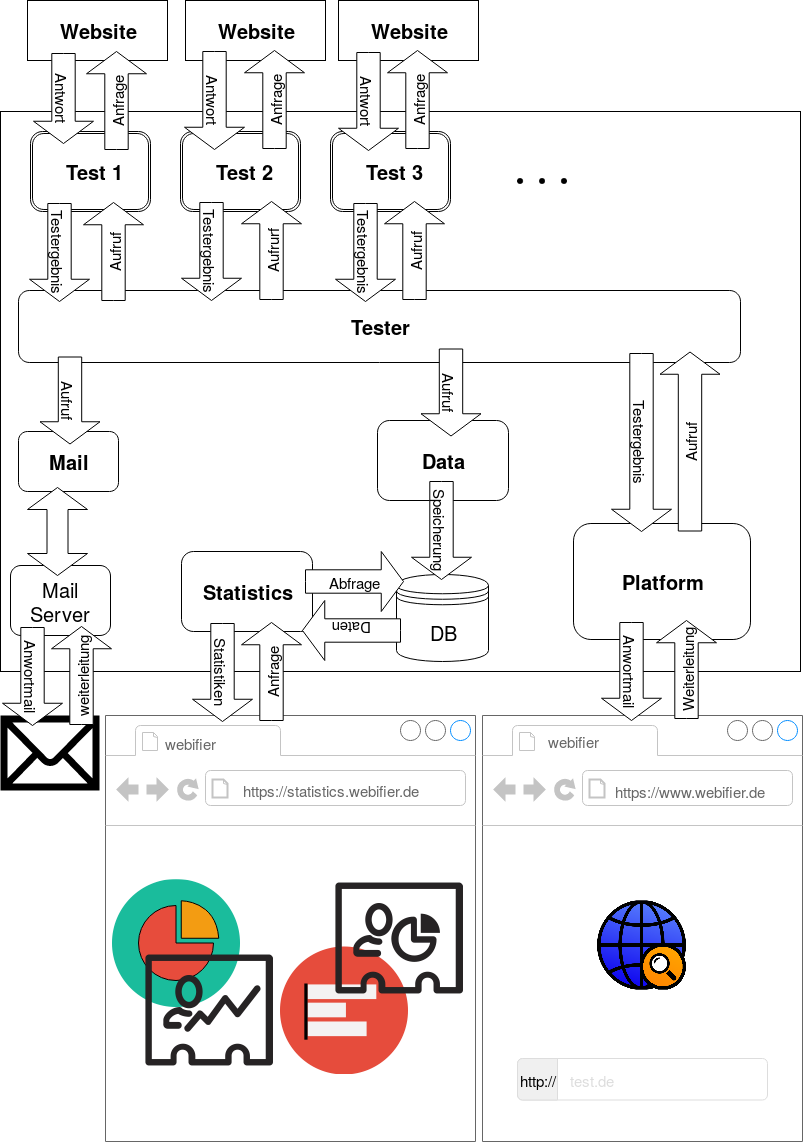
\includegraphics[width=\textwidth]{images/anwendung-konzept}
	\caption{Konzeptarchitektur der Gesamtanwendung}
	\label{fig:anwendung-konzept}
\end{figure}

Grundsätzlich wird webifier benutzt, um Webseiten auf verschiedene Sicherheitsaspekte zu untersuchen.
Abbildung \ref{fig:anwendung-konzept} zeigt den groben Plan der Anwendung.
Es zeigt den konzeptionellen Zusammenhang zwischen den Komponenten, wobei die Datenbank und der Mail Server nicht als eigene Komponenten entwickelt wurden und deshalb keine eigenen Unterabschnitte erhalten.
Die Aufnahme der URLs erfolgt über eine Webseite, die von der Plattform an den Browser des Nutzers ausgeliefert wird.
Die Platform leitet die \ac{URL} aus der Nutzeranfrage an dann an den Tester weiter.
Der Tester ist die Komponente, die die \ac{URL} auf Korrektheit überprüft und ggf. Weiterleitungen auflöst.
Entsteht dabei ein Fehler, so wird dieser an die Platform porpagiert und schließlich im Browser angezeigt.
Wurde die Auflösung der \ac{URL} erfolgreich ausgeführt, werden die Sicherheitstests gestartet.

Eine weitere Möglichkeit, webifier zu verwenden, ist über Mailverkehr.
Hat der Nutzer eine Spam-verdächtige E-Mail in seinem Postfach, so kann er diese an ein bestimmtes Postfach von webifier weiterleiten.
Dort werden Links  aus der Mail zusammengetragen und an den Tester weitergeleitet.

Im Tester wird die Ausführung der einzelnen Tests gestartet, überwacht und koordiniert.
Wichtig dabei ist, dass alle Tests abgeschottet vom Rest des Systems laufen, da auf ihnen schadhafte Webseiten aufgerufen werden.
Es können beliebig viele Tests im Tester hinzugefügt werden, indem sie in der Konfiguration angegeben werden.
Jeder dieser Tests gibt ein eigenes Ergebnis, sowie weitere Informationen zurück.
Diese Ergebnisse werden dann miteinander verrechnet und es wird eine Gesamteinschätzung zusammen mit allen relevanten Informationen der einzelnen Tests ausgegebe.

Alle Ergebnisse der Tests werden anhand von Schwellwerten und Gewichtungen ausgerechnet, wobei die Anwendung zwischen vier Ergebnistypen unterscheidet: \textit{CLEAN}, \textit{SUSPICIOUS}, \textit{MALICIOUS} und \textit{UNDEFINED}.

\begin{description}
    \item[unbedenklich] \hfill \texttt{CLEAN} \\
    Die Webseite verhält sich harmlos und ist ungefährlich.
	\begin{figure}[H]
		\centering
		
\includegraphics[scale=0.2]{images/webifier-clean}
		\caption{Icon für den Testergebnistyp \textit{CLEAN}}
	\end{figure}

	\item[verdächtig] \hfill \texttt{SUSPICIOUS} \\
	Die Webseite verhält sich bedenklich und ist suspekt.
	Diese Seite sollte gemieden werden.
    \begin{figure}[H]
    	\centering
    	
\includegraphics[scale=0.2]{images/webifier-suspicious}
    	\caption{Icon für den Testergebnistyp \textit{SUSICIOUS}}
    \end{figure}

    \item[bedrohlich] \hfill \texttt{MALICIOUS} \\
    Die Webseite verhält sich kritisch und ist gefährlich.
    Sie sollte unter keinen Umständen aufgerufen werden.
    \begin{figure}[H]
    	\centering
    	
\includegraphics[scale=0.2]{images/webifier-malicious}
    	\caption{Icon für den Testergebnistyp \textit{MALICIOUS}}
    \end{figure}

	\item[unbekannt] \hfill \texttt{UNDEFINED} \\
	Der Test konnte aus technischen oder zeitlichen Gründen nicht vollendet werden.
	Es kann keine Aussage über die Bös- oder Gutartigkeit der Seite gemacht werden.
	\begin{figure}[H]
		\centering
		
\includegraphics[scale=0.2]{images/webifier-undefined}
		\caption{Icon für den Testergebnistyp \textit{UNDEFINED}}
	\end{figure}
\end{description}

Das berechnete Gesamtergebnis des Testers wird an die webifier Platform bzw. an webifier
Mail weitergeleitet. Schließlich wird das Ergebnis dem Nutzer über den Browser bzw. über eine
Antwortmail präsentiert. Zusätzlich werden alle Ergebnisse des Testers an webifier Data geschickt
und dort in einer Datenbank persistiert. Diese Daten werden von webifier Statistics für Analysen und
Auswertungen genutzt

\subsection{webifier Tests}
Webifier Tests ist der Oberbegriff für sämtliche von webifier durchgeführten Tests bei der Analyse einer Webseite. Wie bei der gesamten Anwendung wird auch bei den Tests viel Wert auf Modularität gelegt. Jeder Test bildet ein eigenständiges Bauteil, welches nach belieben integriert oder entfernt werden kann ohne Effekte auf die Lauffähigkeit der Gesamtanwendung.

Da webifier auf die Analyse von maliziösen Seiten ausgelegt ist gibt es bei den Tests einige Punkte zu beachten um das System vor Viren und Schadcode zu schützen.
Jeder Test wird in einer vom Gesamtsystem abgekapselten Laufzeitumgebung ausgeführt. Aus einem Test heraus darf nicht auf das System zugegriffen werden, da die Tests gegebenenfalls mit Schadcode befallen werden können durch das Erforschen von maliziösen Seiten. Es soll vermieden werden, dass sich Schadcode oder Viren von den Tests auf den Server verbreiten. Nach Durchlauf und Übermittelung des Ergebnisses löscht der Test sich selbst und alle Laufzeitdaten. Als Ergebnis werden keinerlei Dateien versendet, es beschränkt sich auf eine Weitergabe des Ergebnisses in Form einer Zeichenkette. Damit soll vermieden werden, dass sich eventuell mit Viren befallene Dateien weiter auf dem System ausbreiten können.

Ein Test liefert sein Ergebnis an den Tester, welcher dies dann im folgenden weiterverarbeitet.
Das Starten und Organisisieren der Tests wird von webifier Tester durchgeführt. Den Aufbau und die Funktionsweise des Testers wird im nächsten Abschnitt beschrieben. Zum Starten eines Tests werden zwei Startparameter mitgegeben. Zum Einen wird die ID zur Identifikation mitgegeben und zum anderen die vollständig aufgelöste URL der zu testenden Seite.
 
Webifier stellt 9 verschiedene Tests um eine Webseite zu überprüfen. Das Konzept der einzelnen Test wird in jeweils eigenständigen Kapiteln erläutert. Hier folgt noch ein Überblick über die einzelnen Tests.

\begin{table}[H]
\centering
\begin{tabular}{|l|l|l|l|}
\hline
\textbf{Test} & \textbf{Beschreibung} \\\hline
Virenscan der Webseite & Testet die Dateien einer Seite auf Viren \\\hline
Vergleich in verschiedenen Browsern & Test ob sich die Seite bei verschiedenen \\ & Browsern anders verhält \\\hline
Überprüfung der Port-Nutzung & Überprüft ob die Seite Portscanning betreibt \\\hline
Überprüfung der IP-Nutzung & Überprüft ob die Seite IPScanning betreibt \\\hline
Prüfung aller verlinkten Seiten & Testet die Links auf der Webseite gegen die \\ & Datenbank von webifier \\\hline
Google Safe Browsing & Nutzt die Google-API um die Webseite von \\ & Google testen zu lassen \\\hline
Überprüfung des SSL-Zertifikats & Überprüft das SSL-Zertifikat der Webseite \\\hline
Erkennung von Phishing & Testet ob es sich um eine Phishingseite handelt \\\hline
Screenshot der Seite & Gibt dem Nutzer einen Screenshot der Webseite \\\hline
\end{tabular}
\caption{Beschreibung der einzelnen Tests}
\label{tbl:tests}
\end{table}

\subsection{webifier Tester}
\label{sec:konzept-tester}

Der webifier Tester verwaltet alle Tests, führt diese aus und berechnet aus den einzelnen Ergebnissen der Tests ein Gesamtergebnis. Alle auszuführenden Tests werden in einer Konfigurationsdatei angegeben und können deshalb dynamisch angepasst werden. Da jeder Test in einem eigenen Prozess läuft wird beim Starten des Testers die Konfigurationsdatei geladen. Anschließend werden die einzelnen Tests ausgeführt und auf ein Ergebnis gewartet. Liegt von allen Tests das Ergebnis vor wird ein Gesamtergebis berechnet. Die Berechnung dieses Ergebnisses wird im Folgenden genauer erklärt.

Das Ergebnis kann entweder unbedenklich (\textit{CLEAN}), verdächtig (\textit{SUSPICIOUS}), bedrohlich (\textit{MALICIOUS}) oder unbekannt (\textit{UNDEFINED}) sein. Für die Berechnung des Endergebnisses erhält jeder Test wie in Tabelle \ref{tbl:test-weights} dargestellt eine Gewichtung, da einige Tests mehr über die Vertrauenswürdigkeit oder Gefahr einer Webseite aussagen als andere. Am meisten fallen der \textit{Virenscan der Webseite} und die \textit{Erkennung von Phishing} ins Gewicht, da dieses die ausschlaggebendsten Tests sind. Am wenigsten gewichtet sind der \textit{Vergleich in verschiedenen Browsern}, weil dies nur ein Indiz ist, da es auch viele Webseiten, wie die von YouTube, Nachrichtensendern, Blogs oder Ähnlichem gibt, welche immer dynamischen Inhalt bereitstellen und die \textit{Prüfung der verlinkten Seiten}, da dies immer vom Datenbestand abhängt. Der \textit{Screenshot der Seite} fällt nicht ins Gewicht, da dies kein Test im eigentlichen Sinne ist, sondern nur eine zusätzliche Information für den Nutzer darstellt. In Abschnitt \ref{sec:konzept-testarten} wird die Wahl der Gewichtungen für die einzelnen Tests noch ausführlicher erläutert.

\begin{table}[H]
\centering
\begin{tabular}{|l|l|l|l|}
\hline
\textbf{Test} & \textbf{Gewichtung} & \textbf{Prozentuale Gewichtung} \\\hline
Virenscan der Webseite & 5 & \textasciitilde0,208\\\hline
Vergleich in verschiedenen Browsern & 1 & \textasciitilde0,042\\\hline
Überprüfung der Port-Nutzung & 3 & 0,125\\\hline
Überprüfung der IP-Nutzung & 3 & 0,125\\\hline
Prüfung aller verlinkten Seiten & 1 & \textasciitilde0,042\\\hline
Google Safe Browsing & 3 & 0,125\\\hline
Überprüfung des SSL-Zertifikats & 3 & 0,125\\\hline
Erkennung von Phishing & 5 & \textasciitilde0,208\\\hline
Screenshot der Seite & 0 & 0\\\hline
\end{tabular}
\caption{Gewichtungen der einzelnen Tests}
\label{tbl:test-weights}
\end{table}

Die prozentuale Gewichtung ergibt sich aus $\frac{Testgewichtung}{Summe~der~Gewichungen~aller~Tests}$.

Ein weiterer wichtiger Punkt, der für die Berechung ges Gesamtergebnisses festgelegt wurde ist, dass mindestens 50\% aller Tests (berechnet anhand der prozentualen Gewichtung) ein bekanntes Ergebnis, also \textit{CLEAN}, \textit{SUSPICIOUS} oder \textit{MALICIOUS} haben müssen. Ist der Anteil bekannter Ergebnisse kleiner lässt sich kein zuverlässiges Ergebnis berechnen, da dieses sonst von zu wenigen ausschlaggebenden Faktoren abhängen würde.

Liefern also mehr als die Hälfte der Tests ein bekanntes Ergebnis, so kann daraus nun das Gesamtergebnis berechnet werden. Hierfür wird für jedes Testergebnis ein Wert zwischen 0 und 1 berechnet, welcher anschließend mit der prozentualen Gewichtung des Tests multipliziert wird. Die Werte der einzelnen Testergebnisse ergeben sich wie in Tabelle \ref{tbl:test-values} dargestellt. Ist das Testergebnis \textit{CLEAN} oder \textit{UNDEFINED} ist der Ergebniswert 0 und geht so nicht weiter in die Wertung ein. Ist das Ergebnis \textit{MALICIOUS} wird der Wergebniswert 1. Dadurch Fällt das Gewicht dieses Tests voll in die Wertung. Ist das Ergebnis \textit{SUSPICIOUS} so wird die prozentuale Gewichtung des Tests als Ergebniswert gewählt. So fließt dieser Test mit dem Quadrat der Gewichtung in das Gesamtergebnis ein.

\begin{table}[H]
\centering
\begin{tabular}{|l|l|l|l|}
\hline
\textbf{Testergebnis} & \textbf{Ergebniswert}\\\hline
\textit{CLEAN} & 0\\\hline
\textit{SUSPICIOUS} & Prozentuale Gewichtung des Tests\\\hline
\textit{MALICIOUS} & 1\\\hline
\textit{UNDEFINED} & 0\\\hline
\end{tabular}
\caption{Zuordnung Testergebnis zu Ergebniswert}
\label{tbl:test-values}
\end{table}

Anschließend werden die Werte aller Tests zu einem Endergebnis aufsummiert. Daraus ergibt sich im Gesamtergebnis ein Minimalwert von 0 und ein Maximalwert von 1. Dieser Wertebereich wird nun wie folgt auf die drei Ergebnisse \textit{CLEAN}, \textit{SUSPICIOUS} und \textit{MALICIOUS} verteilt. Die Tests mit der größten Gewichtung sollen hierbei ausschlaggebend sein. Daraus ergibt sich die prozentuale Gewichtung des Tests mit der größten Gewichtung als Minimalwert für \textit{MALICIOUS} und das Quadrat der prozentualen Gewichtung des Tests mit der größten Gewichtung als Minimalwert für \textit{SUSPICIOUS}.

Daraus lässt sich für die Werte der Tests aus Tabelle \ref{tbl:test-weights} die folgende Werteverteilung der Gesamtergebniswerte ableiten:

\begin{center}
$0 \leq CLEAN < 0,043402\overline{7} \leq SUSPICIOUS < 0,208\overline{3} \leq MALICIOUS \leq 1$
\end{center}

Zusätzlich zu dem berechneten Gesamtergebnis stellt der Tester auch alle Ergebnisse der Einzeltests und deren spezifischen Testinformationen bereit. Außerdem werden alle Ergebnisse zu Persistierung an das Modul webifier Data gesendet, welches in Abschnitt \ref{sec:konzept-data} genauer erläutert wird.

\subsection{webifier Plattform}

webifier Plattform ist eine Webanwendung, die auf den Tester aufsetzt und eine \ac{UI} für diesen zu Verfügung stellt. Außerdem bereitet sie die Ergebnisse des Testers grafisch für den Benutzer auf.

Der Nutzer hat die Möglichkeit auf der ersten Seite von webifier Plattform eine Url einzugeben, welche getestet werden soll. Da die Kapazität jedes Systems beschränkt ist verwaltet die Plattform alle Anfragen zur Webseitenüberprüfung in einer Warteschlange. In einer Konfigurationsdatei kan angegeben werden, wie viele Tests parallel ausgeführt werden sollen. So wird die Warteschlange nach und nach abgearbeit und anschließend werden die Ergebnisse des Testers für den Benutzer visuell aufbereitet. Das bereitgestellte Ergebnis umfasst zum Einen das Gesamtresultat, welches vom Tester berechnet wurde und zu Anderen sowohl die Ergebnisse der einzelen Tests, als auch die Zusätzlichen Informationen, welche von diesen bereitgestellt wurden.

So erhält der Nutzer einen umfassenden Bericht über die Vertrauenswürdigkeit oder die ausgehende Gefahr der überprüften Webseite.

\subsection{webifier Mail}
Diese Komponente ist ein Zusatzfeature, mit dem verdächtige Mails über den webifier Tester überprüft werden können. Nutzer müssen dazu lediglich ihre empfangene Mail an für \textit{webifier Mail} bereitgestelltes Postfach weiterleiten. In \textit{webifier Mail} werden dann bis zu fünf in der Mail enthaltene Links an den Tester weitergeleitet. Ist die Prüfung vollendet wird eine Antwortmail mit den Ergebnissen an den Nutzer zurückgeschickt.

\subsection{webifier Data}
\label{sec:konzept-data}

webifier Data ist die Persistenzkomponente von webifier. webifier Tester nutzt webifier Data um alle Testergebnisse an einem zentralen Ort abzulegen, egal wo dieser ausgeführt wird.

Ein Testergebnis, welches in dem Datamodul gespeichert wird enthält einmal die eingegebene Url und die getestete Url, das Gesamtergebnis, sowohl den Typ (\textit{CLEAN}, \textit{SUSPICIOUS}, \textit{MALICIOUS} oder \textit{UNDEFINED}), als auch den Ergebniswert. Außerdem wird die Testlaufzeit gespeichert. Zusätzlich werden noch weitere Informationen zu den einzelnen Tests gespeichert. Dazu zählen der Name, die Konfigurationsparameter, wie beispielsweise die Gewichtung, das Resultat und die Detailinformationen zu diesem.

Die Komponente stellt auch eine Schnittstelle zum Abfragen der bereits gespeicherten Ergebnisse bereit. Diese wird beispielsweise vom Test \textit{Prüfung aller verlinkten Seiten} verwendet. Die Funktionsweise dieses Tests wird in Abschnitt \ref{sec:konzept-linkchecker} erklärt.

Alle Ergebnisse werden in einer Datenbank abgelegt. Da die zusätzlichen Informationen der einzelnen Tests teilweise sehr unterschiedlich sind, kommt hierfür keine relationale Datenbank in Frage. webifier Data nutzt deshalb zur Speicherung aller Daten die Dokument basierte Datenbank MongoDB. Alle weiteren Informationen hierzu folgen im Umsetzungsteil dieser Arbeit.

\subsection{webifier Statistics}
Webifier Statistics ist die Statistikoberfläche von webifier. Hier werden alle Daten der analysierten Webseiten aufbereitet und in visueller Form dargestellt. Die Daten stammen aus den Ergebnissen aller Tests, welche von webifier Data abgespeichert wurden.

Webifier Statistics liefert dem Nutzer eine Vielzahl an verschiedenen Graphen, welche bestimmte Teilaspekte beleuchten. Diese enthalten zum Einen die Gesamtauswertungen, welche sich mit der allgemeinen Datenauswertung jedes Gesamttests beschäftigen. Zum Anderen gibt es noch die Einzelauswertungen der Tests, die testspezifische Ergebnisse auswerten.

Alle Auswertungen werden dem Nutzer über eine Weboberfläche zugänglich gemacht. Als Einstieg gibt es ein \textit{Dashboard} mit einigen Zahlen und Fakten zu den Aktivitäten auf webifier. Auf die einzelnen Auswertungen wird in der Auswertung genauer eingegangen.

\section{Testarten}
\label{sec:konzept-testarten}

In diesem Abschnitt werden nun die einzelnen Tests vorgestellt, mit welchen die zu überprüfende Webseite analysiert wird. Wie bereits erwähnt werden alle dieser Tests vom Tester verwaltet und ausgeführt.

\subsection{Virenscan der Webseite}

Der Virenscan der Webseite führt nutzt verschiedene Virenscanner um die Webseite auf Malware zu überprüfen. Um dies zu realisieren wird zunächst die Webseite inklusive aller enthaltenen Dateien und Links heruntergeladen und gespeichert. Anschließend werden die Virenscanner gestartet, welche die heruntergeladenen Dateien überprüfen. Abschließend werden alle Ergebnisse der einzelnen Scans zusammengeführt und daraus ein Endergebnis berechnet.

Für das Endergebnis werden zunächst alle gescannten Dateien klassifiziert. Wird eine Datei von keinem der Virenscanner als Malware eingestuft wird diese als \textit{CLEAN} gekennzeichnet. Klassifiziert nur ein Virenscanner die Datei als Malware, wird diese also \textit{SUSPICIOUS} eingestuft. Halten mehr als ein Virenscanner eine Datei für Malware ist diese \textit{MALICIOUS}. Sind alle Dateien als \textit{CLEAN} eingestuft, so ist auch das Endergeblis dieses Tests \textit{CLEAN}. Sollten ein oder mehrer Dateien \textit{SUSPICIOUS} sein wird auch das Endergebnis \textit{SUSPICIOUS}. Das selbe gilt danach für \textit{MALICIOUS}. Sobald eine Datei \textit{MALICIOUS} ist, ist das Endergbnis ebenfalls \textit{MALICIOUS}.

Zusätzlich zum Endergebnis wird noch die gesamte Liste der gescannten Dateien inklusive der jeweiligen Klassifizierung bereitgestellt und vom Tester weitergegeben.

\subsection{Vergleich in verschiedenen Browsern}

In \autoref{sec:user-agent-sniffing} wurde bereits das Thema \textit{User Agent Sniffing} behandelt.
Dieser Test soll genau dieses Problem aufgreifen.
Es sollen \ac{HTTP}-Anfragen von verschiedene Browsertypen mit entsprechenden User Agents an den Webserver der Zielseite geschickt werden.
Danach werden die Antworten untereinander auf Unterschiede untersucht. Dabei entstehen Kennwerte für die Übereinstimmung der Antworten, die miteinander verrechnet werden müssen.
Dieser berechnete Wert für die Durchschnittsübereinstimmung muss schließlich anhand von passenden Schwellwerten die richtige Ergebnisklasse eingeteilt werden.

\subsection{Überprüfung der Port-Nutzung}
Der Test auf Port Scanning analysiert die Nutzung der Ports einer Webseite. Hierfür wird die Webseite automatisch vom Test geöffnet und dessen JavaScript ausgeführt. Parallel dazu muss die Netzwerkaktivität überwacht werden. Es werden alle eingehenden Anfragen auf das Testsystem zunächst geloggt. Da das Testsystem abgekapselt vom restlichen System ist, ist es irrelevant von welcher IP-Adresse die Anfragen kommen. Alle Anfragen lassen sich auf die aufgerufene Seite zurückführen, da restliche Netzwerkaktivität abgeschaltet ist. Dies ist wichtig, da es durchaus möglich ist das die Webseite nicht selbst einen Portscan-Angriff startet sondern beispielsweise über einen Drittrechner oder ein Botnetz gescannt wird. Zudem könnten die Ports auch lokal auf dem Client über JavaScript gescannt werden. Deshalb werden lediglich die angefragten Ports im Log gespeichert.

Nach erfolgreichem Durchschauen der Webseite beginnt die Analyse. Hier müssen alle Portanfragen klassifiziert werden. Es gibt eine Reihe von legitimen Portanfragen welche beispielsweise Port 80 für HTTP oder Port 443 für SSL sind. Diese Anfragen werden dann als harmlos markiert und somit ignoriert. Alle Anfragen, welche sich auf unspezifizierte Ports beziehen, werden als verdächtig markiert. Je nach Anzahl der verdächtigen Anfragen wird dann entschieden ob die Seite als bedrohlich, verdächtig oder sauber klassifiziert wird. Dieses Ergebnis wird dann mitsamt der gefundenen verdächtigen Portanfragen zurückgegeben.

\subsection{Überprüfung der IP-Nutzung}
Der Test auf IP Scanning beschäftigt sich mit der Analyse der IP-Anfragen, welche durch eine Webseite ausgelöst werden. Wie auch bereits bei Portscanning beschrieben wird die Webseite automatisch geöffnet und dessen JavaScript ausgeführt. Die Netzwerküberwachung hat hier jedoch einen anderen Fokus. Es werden die IPs der gesendeten Anfragen geloggt. Beim IP Scanning wird grundsätzlich versucht über die bekannten Heimnetz-IP-Netze weitere im Netzwerk angeschlossene Geräte zu erkennen um beispielsweise Viren auf dem gesamten Netzwerk zu verbreiten. Diese Angriffe werden über JavaScript auf dem Clienten gestartet. Deshalb werden die vom Clienten gesendeten Anfragen protokolliert. Hiervon werden lediglich die IPs gespeichert.

Nach dem Speichern aller IPs werden diese klassifiziert. Der Test vergleicht alle Anfragen mit den bekannten Heimnetz-IPs (beispielsweise 192.168.178.*). Anfragen, welche sich nicht auf diese Adressen zurückführen lassen werden herausgefiltert, da diese irrelevant für den Test sind. Anhand der Anzahl der verdächtigen Adressen wird im Abschluss wieder die Seite klassifiziert und das Ergebnis mitsamt den Adressen zurückgeliefert an den Tester.

\subsection{Prüfung aller verlinkten Seiten}
\label{sec:konzept-linkchecker}

Dieser Test sucht innerhalb des Quellcodes der Anwendung nach Hyperlinks und referenzierten Ressourcen.
Für alle gefundenen Hosts wird dann prüft, ob bereits Einträge dazu in der Datenbank unter webifier Data vorhanden sind.
Gibt es einen Eintrag, der \textit{SUSPICIOUS} ist, dann ist das ganze Endergebnis \textit{SUSPICIOUS}.
Falls jedoch mehr als 34\% der Hosts \textit{UNDEFINED} sind, dann ist auch das Gesamtergebnis \textit{UNDEFINED}.
Sobald ein Eintrag \textit{MALICIOUS} ist, so ist auch das Gesamtergebnis \textit{MALICIOUS}.
Ansonsten liefert der Test \textit{CLEAN} zurück.

\subsection{Google Safe Browsing}

\begin{quote}
	Safe Browsing is a Google service that lets client applications check URLs against Google's constantly updated lists of unsafe web resources.\footcite[Vgl.][]{googleSafeBrowsing}
\end{quote}

Dieser Cloud-Service erlaubt es der Anwendung also eine weitaus größere Datenbank als ihre eigene anzuzapfen.

Der Service unterscheidet zwischen vier Bededrohungstypen\label{par:konzep-gsb-types}: Malwareseiten, Sozialmanipulationsseiten, ungewollte Software und potenziell schadhafte Webanwendungen.
Weitere Vorteile sind die Autorität des Unternehmens und die einfach zu bewerkstelligende Integration des Services.
Leider können die Einträge aus der Datenbank des Services nicht exportiert werden, sondern können nur gegen Listen von Links gecheckt werden.
In diesem Test werden wie bei der Prüfung der verlinkten Seiten alle Links zu Webseiten und Resourcen zusammengetragen.
Diese werden dann aber nicht an webifier Data, sondern an den Google Safe Browsing Dienst weitergeleitet.
Sobald ein Treffer aus dem Service zurückgemeldet wird, ist das Ergebnis \textit{SUSPICIOUS}.
Falls sich mehr als 40\% der Links in der Datenbank befinden, so wird die Webseite als \textit{MALICIOUS} eingestuft.
Ist die zu testende Webseite selbst ein Match, so ist das Ergebnis ebenfalls \textit{MALICIOUS}.
Wird kein Eintrag gefunden, dann zählt die Seite als \textit{CLEAN}.

\subsection{Überprüfung des SSL-Zertifikats}

Die Überprüfung des SSL-Zertifikats der Weibseite sucht nach einem vorhandenen Zertifikat und validiert dieses, sofern die Webseite eines nutzt. Hierfür liest es die dafür notwendigen Informationen des  Zertifikats aus und berechnet anschließend ein Testergebnis.

Stellt die Webseite kein Zertifikat zur Verfügung so ist das Testergebnis \textit{SUSPICIOUS}, da es in Zeiten von Let's Encrypt\footnote{\url{https://letsencrypt.org/}} jedem möglich ist ein SSL-Zertifikat kostenlos zu erwerben und so die Sicherheit der eigenen Webseite zu erhöhen. Nutzt die Webseite ein valides Zertifikat ist das Ergebnis \textit{CLEAN}. Weist das Tertifikat Fehler auf ist das Ergebnis \textit{MALICIOUS}. Solche Fehler können beispielsweise sein, dass das Zertifikat abgelaufen ist, dass es selbst signiert wurde oder das es für den falschen Host genutzt wird.

\subsection{Erkennung von Phishing}

webifier enthält auch einen sehr einfachen Test zur Erkennung von Phishing. Dieser sucht zuerst nach den Schlagwörtern der gegebenen Webseite. Hierfür zählt er die Häufigkeit aller vorkommenden Wörter die mehr als drei Buchstaben haben. Wörter in Bildbeschreibungen und Überschriften werden doppelt gewichtet, Wörter im Titel der Webseite werden fünffach gewichtet. Haben mehere Wörter die gleiche Gewichtung, so fällt die Länge der Wörter auch noch ins Gewicht und längere Wörter werden bevorzugt. Die vier Wörter, die im Ranking am höchsten stehen werden anschließend als Schüsselwörter gewählt.

Anschließend werden mit Hilfe öffentlicher Suchmaschinen mögliche Duplikate der Webseite gesucht. Für diese Suche werden die ausgewählten Schlagwörter verwendet. Nun werden die Ergebnisse aller Suchmaschinen zusammengeführt und ebenfalls gewichtet. Je mehr Suchmaschinen einen Link gefunden haben, desto höher steigt dieser Link im Ranking. Als nächstes muss diese Liste der möglichen Duplikate nach Orginalen, welcher der gegebenen Webseite entsprechen gefilterert werden, da es sehr wahrscheinlich ist, dass diese ebenfalls in der Liste der Links enthalten ist. Als letztes wird die Liste noch auf maximal zehn Eintrage gekürtzt.

Nun werden alle gefundenen Links mit der gegebenen Webseite verglichen und für jeden gefundenen Link ein Ergebnis berechnet. Der Vergleich erfolgt auf drei Ebenen: es werden der Inhalt und er der Quelltext der beiden Webseiten, aber auch das Aussehen verglichen. Jeder dieser Vergleiche gibt die prozentuale Übereinstimmung der zu vergleichenden Webseiten zurück. Anschließend werden diese drei Ergebnisse zu einem Gesamtergebnis verrechnet. In diese Rechnung fließt das Ergebnis des Screenshotsvergleichs mitt doppeltem Gewicht ein, da dieser Vergleich am aussagekräftigsten ist.

Aufgrund der Komplexität wird die genaue Berechnung des Ergebnisses wird in Abschnitt \ref{sec:umsetzung-phishungdetector} erklärt und hier nun vereinfacht dargestellt. Stimmen die beiden Webseiten zu 80\% überein, so ist das Ergebnis des Links \textit{SUSPICIOUS}, stimmen die beiden Webseiten zu 90\% überein, so ist das Ergebnis \textit{MALICIOUS}. Das Endergebnis des Tests wird abschließend wie folgt berechnet: wurde mindestens ein verdächtiger Link gefunden, so ist das Gesamtergebnis \textit{SUSPICIOUS}, wurde mindestens ein bedrohlicher Link gefunden, so ist das Ergebnis \textit{MALICIOUS}, andernfalls \textit{CLEAN}. Zusätzlich werden noch die gefundenen Schlagwörter, die gefundenen Phishingseiten, derern Vergleichswerte und ein Überlagerungsscreenshot mit der Originalseite für den Tester bereitgestellt.

\subsection{Screenshot der Seite}
Der Screenshot-Test ist kein Test im eigentlichen Sinne. Er liefert keine Aussage über die Bedrohlichkeit einer Webseite. Deshalb liefert er immer als Ergebnis sauber und bleibt ungewichtet in der Gewichtung im Tester. Trotzdem wurde er mit implementiert um den Nutzern einen Blick auf die Seite zu geben, welche sie von webifier haben scannen lassen. Dies kann besonders interessant sein, da viele Nutzer auch daran interessiert sind wie die Seiten denn aussehen und was dort an Text oder Bilder zu sehen ist. Jedoch sollte keiner der Nutzer, auf eine als bedrohlich markierte Webseite, mit seinem Webbrowser zugreifen. Deshalb wird hier die Möglichkeit gegeben sich gefahrlos einmal die Webseite anzuschauen.

\chapter{Umsetzung}

In diesem Kapitel wird nun aufbauend auf dem im vorherigen Kapitel beschriebenen Konzept die Umsetzung von webifier beschrieben. Zunächst folgt nun die Erläuterung der Gesamtumsetzung, gefolgt von der Umsetzung der Teilanwendungen. Abschließend wird die Implementierung der einzelnen Tests vorgestellt.

\section{Gesamtanwendung}

\todo{Daniel}

\subsection{webifier Tests}
In diesem Abschnitt wird der allgemeine Aufbau, welcher für alle Tests von webifier gilt, erläutert.

Um die Tests vom Gesamtsystem abzukapseln wird auf Docker gesetzt. Hierbei wird für jeden Test ein eigenes Image geschrieben. Die Tests werden vom Tester dann gestartet. So wird jeder Test in einem eigenen Container ausgeführt. So ist sichergestellt, dass die Tests unabhängig von äußeren Faktoren sind und sich gegenseitig oder das Gesamtsystem nicht beeinflussen.

Die Technologien der einzelnen Tests sind abhängig vom jeweiligen Test und werden deshalb in den jeweiligen Kapiteln erläutert. Die Ergebnisübermittelung der Tests an den Tester wird mittels \ac{JSON}-Strings realisiert. Wie in Beispiel (...) zu sehen besteht das \ac{JSON} aus dem Testergebnis und einer ResultInfo. Die ResultInfo varriert von Test zu Test. Hier können für jeden Test weitergehende Informationen übermittelt werden. Für den Test auf Portscanning wird beispielsweise eine Liste von verdächtigen Portanfragen übermittelt.

\begin{scriptsize}
\lstset{
    style=eclipsejavascript,
    caption={Result JSON},
    label={lst:resultjson}
}
\begin{lstlisting}
  {
  	"result": "clean" | "suspicious" | "malicious" | "undefined",
  	"info": {
  		...
  	}
  }
\end{lstlisting}
\end{scriptsize}

\begin{itemize}
  \item Beschreiben der Startparameter URL und ID
\end{itemize}

\subsection{webifier Tester}

Der webifier Tester wurde als Anwendung für das \ac{CLI} in Java implementiert. Der Tester kann mit Hilfer verschiedener Parameter in seinem Verhalten gesteuert werden. Die Option \lstinline[style=eclipse]{-h} gibt beispielsweise die in Listing \ref{lst:tester-help} dargestellte Hilfe aus.

\begin{scriptsize}
\lstset{
    style=eclipse,
    caption={Hilfe webifier Tester},
    label={lst:tester-help}
}
\begin{lstlisting}
usage: java -jar webifier-tester.jar
 -h,--help              Print this help screen.
 -i,--id <ID>           Set the id for this test
 -o,--output <FORMAT>   Set the format of the output. Valid formats are
                        JSON and XML.
 -u,--url <URL>         The url that should be tested.
\end{lstlisting}
\end{scriptsize}

Die einzig erforderliche Option ist \lstinline[style=eclipse]{-u} mit welcher die zu überprüfende Url angegeben wird. Mit der Option \lstinline[style=eclipse]{-i} kann dem Test eine Id gegeben werden. Wird keine Id angegeben generiert der Tester eigenständig eine Id für den gestarteten Test. Mit der Option \lstinline[style=eclipse]{-o} kann ein Ausgebaformat spezifiziert werden. Dies ist vorallem für die automatisierte Testausführung, beispielsweise mit webifier Plattform relevant. Mögliche Ausgabeformate sind \ac{JSON} und \ac{XML}. Ist ein Ausgabeformat angegeben werden alle Events (Start und Ende der Tests) im jeweiligen Format ausgegeben. Wird kein Format spezifiziert so werden die Ergebnisse wie in Listing \ref{lst:tester-result} dargestellt ausgegeben.

\begin{scriptsize}
\lstset{
    style=eclipse,
    caption={Standardausgabe webifier Tester},
    label={lst:tester-result}
}
\begin{lstlisting}
$ java -jar webifier-tester.jar -u securitysquad.de
Resolver started for url securitysquad.de
Resolver finished! Result:
The resolved url is 'https://www.securitysquad.de/' and it is reachable.
Start Tester for url https://www.securitysquad.de/
Test 'VirusScan' started!
Test 'PhishingDetector' started!
Test 'CertificateChecker' started!
Test 'Screenshot' started!
Test 'IpScan' started!
Test 'GoogleSafeBrowsing' started!
Test 'LinkChecker' started!
Test 'PortScan' started!
Test 'HeaderInspection' started!
Test 'CertificateChecker' finished! Result:
The given url is clean!
Test 'HeaderInspection' finished! Result:
The given url is clean!
Test 'Screenshot' finished! Result:
The given url is clean!
Test 'GoogleSafeBrowsing' finished! Result:
The given url is clean!
Test 'LinkChecker' finished! Result:
The test result is undefined. Maybe the test returned an error!
Test 'IpScan' finished! Result:
The given url is clean!
Test 'PortScan' finished! Result:
The given url is clean!
Test 'PhishingDetector' finished! Result:
The given url is clean!
Test 'VirusScan' finished! Result:
The given url is clean!
Tester finished for url https://www.securitysquad.de/
The url is clean!
\end{lstlisting}
\end{scriptsize}

Wie im Konzept bereits erwähnt verwaltet der Tester alle auszuführenden Tests. Um die Tests dynamisch anpassen zu können werden alle notwendigen Parameter in einer Konfigurationsdatei gespeichert. Listing \ref{lst:tester-config} zeigt einen Ausschnitt dieser Datei.

Jeder Test hat einen eindeutigen Namen, seine Gewichtung, ein Befehl zum Ausführen und zum Beenden des Tests, sowie dafür vorgesehene Timeoutzeiten in Sekunden. Außerdem hat jeder Test einen Parameter, welcher die Java-Klasse für das Testergebnis angibt und einen Parameter mit dem der Test aktiviert oder deaktiviert werden kann. Bei der Ausführung und beim Beenden der Tests werden die Platzhalter \lstinline[style=eclipse]{#ID} und \lstinline[style=eclipse]{#URL} durch die generierten, bzw. vom Nutzer angegebenen Daten ersetzt.

\begin{scriptsize}
\lstset{
    style=eclipsejavascript,
    caption=[Ausschnitt Konfigurationsdatei webifier Tester]{Ausschnitt Konfigurationsdatei webifier Tester\protect\footnotemark},
    label={lst:tester-config}
}
\begin{lstlisting}
{
  "resolver": {
    "name": "resolver",
    "startup": "docker run --rm --name #ID -e URL=#URL -e ID=#ID webifier-resolver",
    "startup_timeout_seconds": 60,
    "shutdown": "docker stop #ID",
    "shutdown_timeout_seconds": 30
  },
  "tests": [
    {
      "name": "VirusScan",
      "startup": "docker run --rm --name #ID -e URL=#URL -e ID=#ID webifier-test-virusscan",
      "startup_timeout_seconds": 600,
      "shutdown": "docker stop #ID",
      "shutdown_timeout_seconds": 30,
      "result_class": "de.securitysquad.webifier.output.result.virusscan.TestVirusScanResultInfo",
      "weight": 5,
      "enabled": true
    }
    ...
  ],
  "preferences": {
    "push_result_data": true
  }
}
\end{lstlisting}
\end{scriptsize}
\footnotetext{Der vollständige Inhalt der Konfigurationsdatei befindet sich in Anhang \appref{b}.}

Am Ende der Datei lässt sich noch die Einstellung festlegen, ob das Endergebnis an webifier Data gesendet werden soll oder nicht. Am Anfang der Datei lässt sich der so genannte \textit{Resolver} konfigurieren. Dieser Prüft vor allen anderen Tests ob die angeforderte Seite überhaupt erreichbar ist und löst wenn nötig Weiterleitungen der Url auf und gibt das Ergebnis an den Tester zurück.

Ist die angegebene Url erreichbar wird die vom \textit{Resolver} aufgelöste Url verwendet und alle anderen Tests damit gestartet. Nun wartet der Tester bis alle Ergebnisse der Tests verfügbar sind oder die Angegebenen Timeouts erreicht sind. Im Falle eines Timeouts erhält der Test das Ergebnis \textit{UNDEFINED}. Abschließend wird das Gesamtergebnis für die angegebene Url wie bereits in Abschnitt \ref{sec:konzept-tester} beschrieben berechnet. Listing \ref{lst:tester-testresult-calculation} zeigt einen Ausschnitt der Implementierung der Ergebnisberechnung.

\begin{scriptsize}
\lstset{
    style=eclipsejava,
    caption=[Ausschnitt Ergebnisberechnung webifier Tester]{Ausschnitt Ergebnisberechnung webifier Tester\protect\footnotemark},
    label={lst:tester-config}
}
\begin{lstlisting}
private WebifierOverallTestResult calculateOverallResult() {
    ...
    if (undefinedPercentage > #MAX_UNDEFINED_TEST_PERCENTAGE#) {
        return new WebifierOverallTestResult(WebifierResultType.##UNDEFINED##);
    }
    double result = 0;
    for (WebifierTest<TestResult> test : tests) {
        double testWeight = (double) test.getData().getWeight() / (double) weightSum;
        result += getTestResultValue(test.getResult().getResultType(), testWeight) * testWeight;
    }
    if (result >= maliciousMin) {
        return new WebifierOverallTestResult(WebifierResultType.##MALICIOUS##, result);
    }
    if (result >= suspiciousMin) {
        return new WebifierOverallTestResult(WebifierResultType.##SUSPICIOUS##, result);
    }
    return new WebifierOverallTestResult(WebifierResultType.##CLEAN##, result);
}
\end{lstlisting}
\end{scriptsize}
\footnotetext{Der vollständige Inhalt der Ergebnisberechnung befindet sich in Anhang \appref{c}.}

Nachdem alle Tests ausgeführt wurden und das Gesamtresultat zusammengefasst wurde wird dieses über die von webifier Data bereitgestellte Schnittstelle dort gespeichert. Die Kommunikation mit webifier Data läuft ebenfalls über das \ac{JSON}-Format. Genaueres hierzu folgt in Abschnitt \ref{sec:umsetzung-data}.

\subsection{webifier Plattform}

In diesem Abschnitt wird nun die Umsetzung von webifier Plattform berschrieben. Diese Komponente wurde mit Java umgesetzt und basiert auf dem Spring-Framework. Zusätzlich kamen im Frontend die Technologiern \ac{HTML}, \ac{CSS} und JavaScript, sowie die Bibliotheken Bootstrap und jQuery zu Einsatz. Zunächst wird nun das Backend beschrieben, danach wird die Oberfläche der Plattform vorgestellt.

webifier Plattform ist eine Webanwendung und bietet eine benutzerfreundliche Öberfläche zur Bedienung von webifier Tester. Um die Plattform für die optimale Nutzung des Testers zu konfigurieren gibt es die in Listing \ref{lst:platform-config} dargestellte Datei, mit der alle notwendigen Parameter angepasst werden können.

\begin{scriptsize}
\lstset{
    style=eclipsejavascript,
    caption={Konfigurationsdatei webifier Plattform},
    label={lst:platform-config}
}
\begin{lstlisting}
{
  "tester": {
    "command": "java -jar webifier-tester.jar -u #URL -i #ID -o JSON",
    "timeout": 15,
    "parallel": 1
  }
}
\end{lstlisting}
\end{scriptsize}

Zunächst muss in der Konfigurationsdatei der Befehl zur Ausführung des Testers angegeben werden. Standartmäßig sollte der Tester im selben Verzeichnis liegen wie die Plattform. Ist dies nicht der Fall, muss der Pfad der Datei entsprechend geändert werden. Außerdem kann ein Timeout für den Tester angegeben werden. Standardmäßig liegt dieses bei 15 Minuten. Der wahrscheinlich wichtigste Parameter zur optimale Nutzung der vorhandenen Ressourcen ist der letzte Parameter. Mit diesem kann angegeben werden wie viele Tests parallel ausgeführt werden sollen. Per default werden alle Tests sequentiell ausgeführt. Wird die Plattform auf einem leistungsstarken System betrieben kann die anzahl entsprechend der vorhandenen Ressourcen angepasst werden.

Die Plattform stellt außerdem eine Möglichkeit zur Massenüberprüfung von Webseiten zur Verfügung. Hierfür kann eine Liste von Urls in form eines Texts oder einer Datei angegeben werden. In diesem Modus ist es allerdings nicht möglich alle Ergebnisse dierekt zu sehen, da der Vorgang je nach größe der Liste mehrere Tage oder Wochen dauern kann. Deshalb ist dieser Modus eher für langfristige Analysen geeignet.

Im Folgenden wird nun noch einmal der Ablauf einer Überprüfung beschrieben und die Oberfläche von webifier Plattform dargestellt. Besucht der Nutzer die Webseite der PLattform sieht er zunächst die in Abbildung \ref{fig:platform-start} gezeigte Startseite. Hier kann der User nun eine beliebige Url in das Eingabefeld tippen und anschließend die Überprüfung starten. Außerdem bietet die Startseite Links zur bereits beschriebenen Batchverarbeitung und zu webifier Statistics. Dieses Modul wird in Abschnitt \ref{sec:umsetzung-statistics} ausführlich dargestellt wird.

\begin{figure}[H]
  \centering
  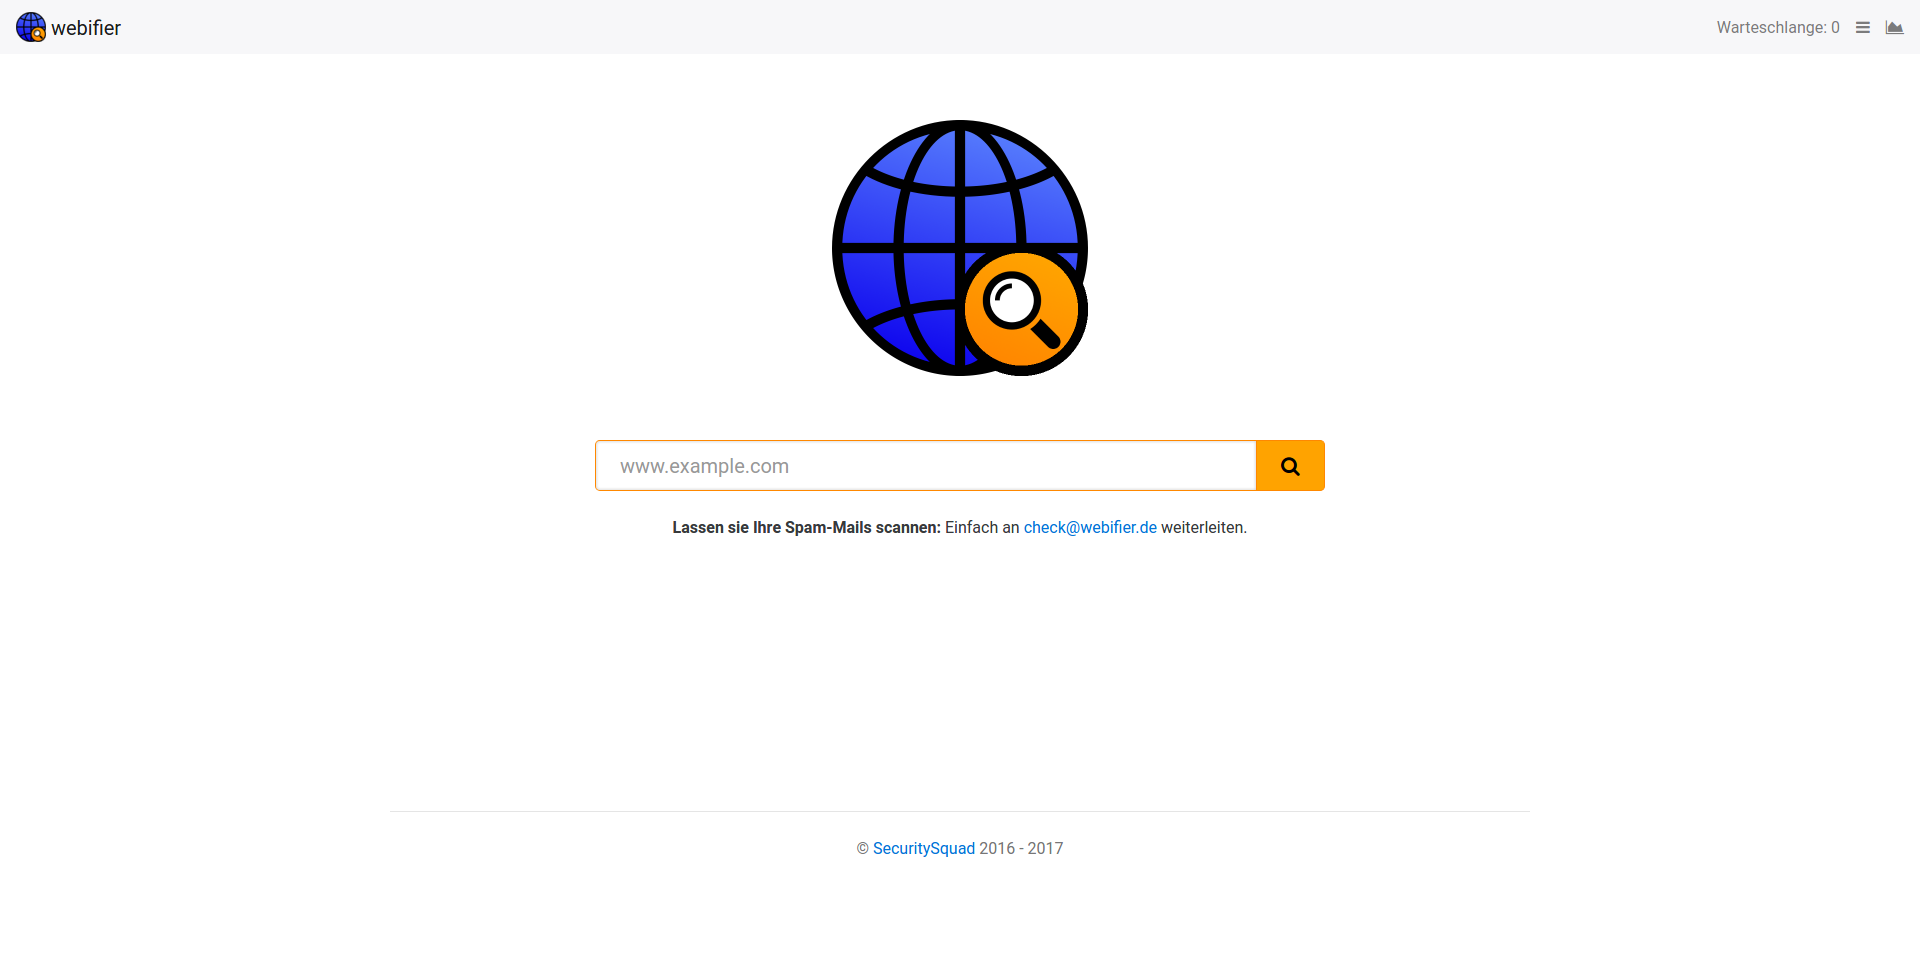
\includegraphics[width=\textwidth]{images/platform/screenshot-start}
  \caption[webifier Platform - Startseite]{webifier Platform - Startseite\protect\footnotemark}
  \label{fig:platform-start}
\end{figure}
\footnotetext{Die Abbildung befindet sich in besserer Qualität in Anhang \appref{d}.}

Nachdem die Überprüfung einer Webseite gestartet wurde wird der Nutzer auf die in Abbildung \ref{fig:platform-result} abgebildete Seite geleitet, welche sich nach und nach mit den Ergebnissen der einzelnen Tests füllt, sobald diese vorliegen. Sind alle Tests beendet, wird auch das Endresultat angezeigt. Die Ergebnisseite bietet zunächst einen kompakten Überblick über alle ausgeführten Tests und deren Ergebnisse.

\begin{figure}[H]
  \centering
  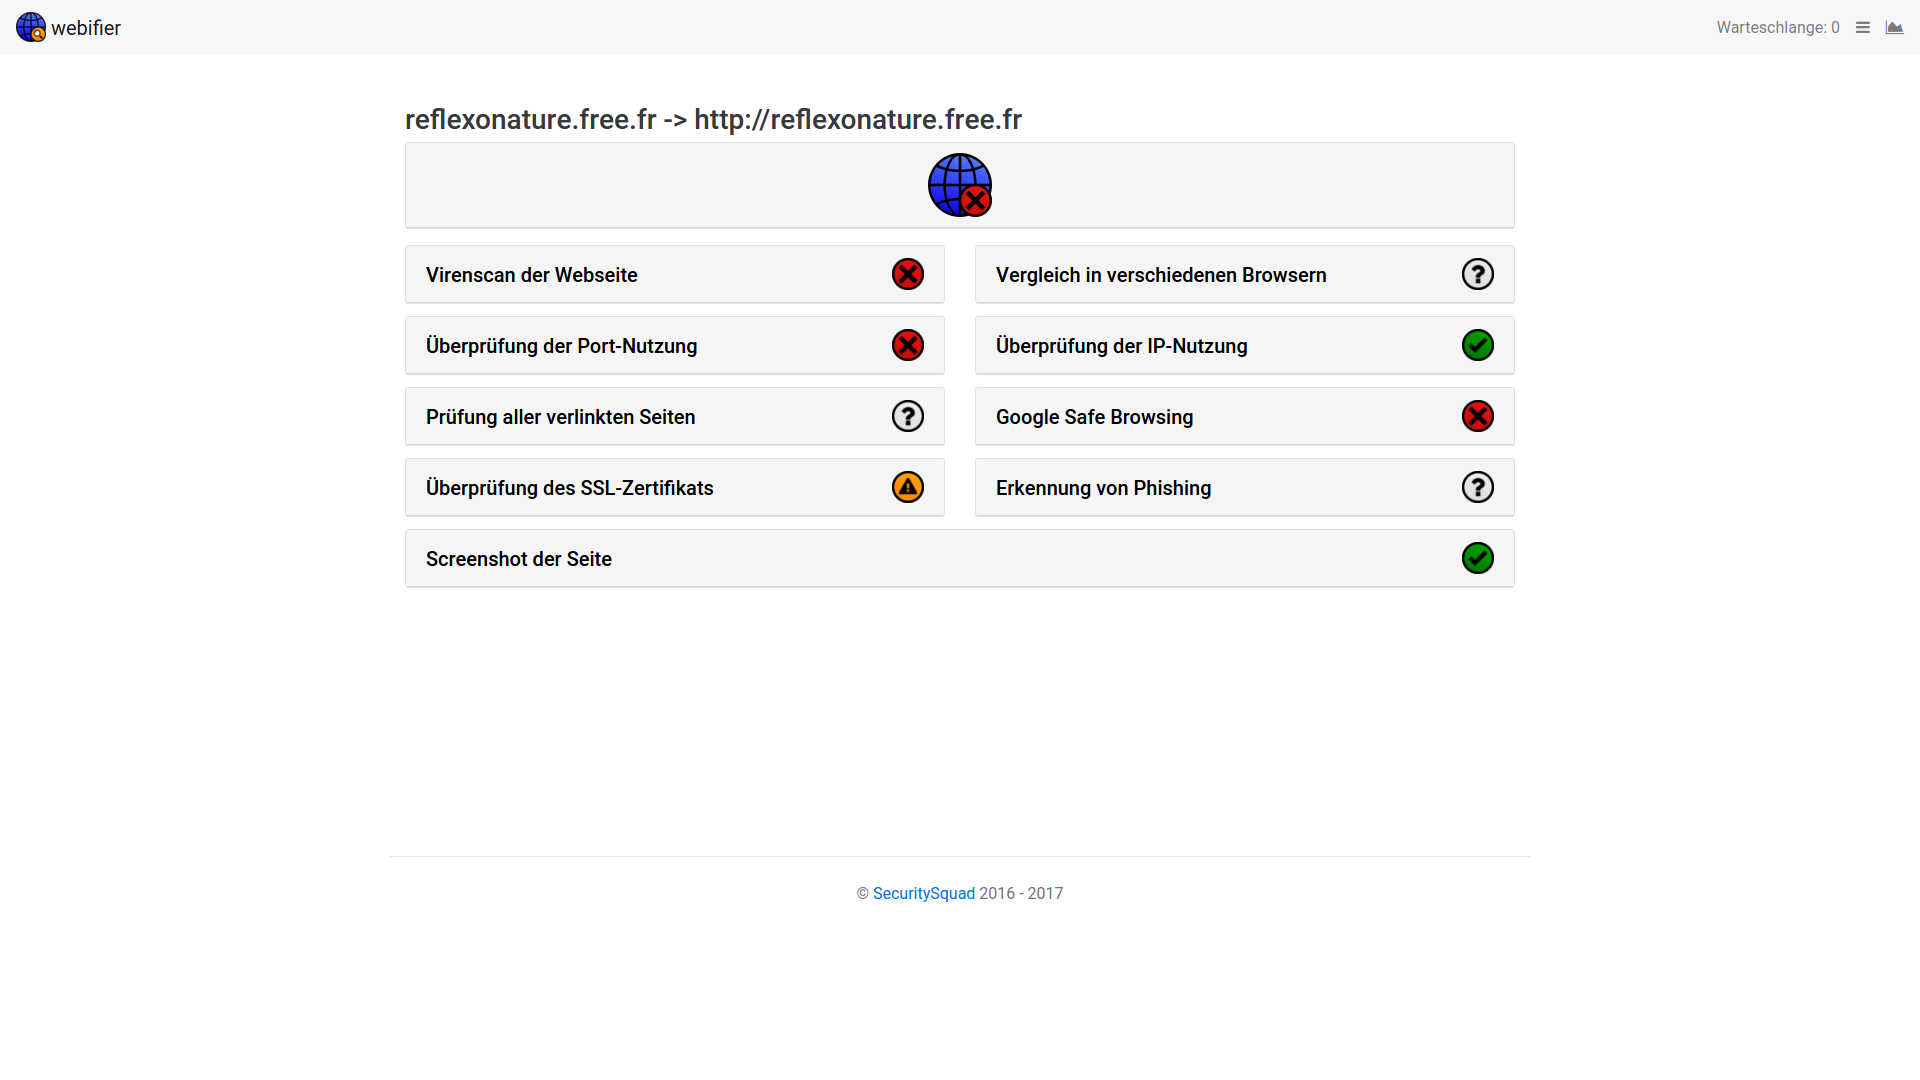
\includegraphics[width=\textwidth]{images/platform/screenshot-reflexonature}
  \caption[webifier Platform - Ergebnisseite]{webifier Platform - Ergebnisseite\protect\footnotemark}
  \label{fig:platform-result}
\end{figure}
\footnotetext{Diese und weitere Ergebnisseiten befinden sich in besserer Qualität in Anhang \appref{d}.}

Möchte der Nutzer noch genauere Informationen zu den Ergebnissen eines Tests, so lassen sich alle Testfelder mit einem Klick darauf ausklappen. Im Folgenden werden nun die Detailansichten der einzelnen Testergebnisse gezeigt und erläutert.

\begin{figure}[H]
  \centering
  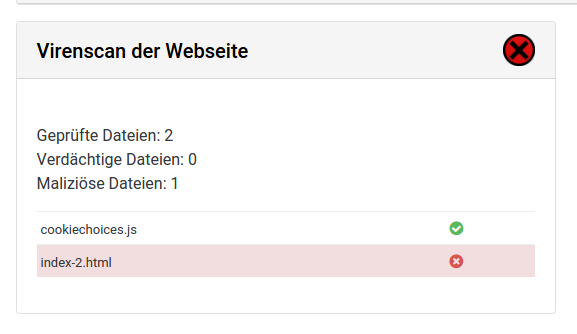
\includegraphics[width=7.5cm]{images/platform/virusscan-malicious}
  \caption{webifier Platform - Virenscan der Webseite}
  \label{fig:platform-result-virusscan}
\end{figure}

Die Detailansicht des Virenscans, welche in Abbildung \ref{fig:platform-result-virusscan} dargestellt ist, zeigt einmal die Anzahl aller gescannten Dateien, sowie die Anzahlen der gefundenen verdächtigen oder maliziösen Dateien. Außerdem erhält die Ansicht eine genaue Auflistung aller Dateien mit entsprechendem Ergebnis. So lässt sich genau feststellen, welche Dateien welche Bedrohung darstellen.

\begin{figure}[H]
\centerline{%
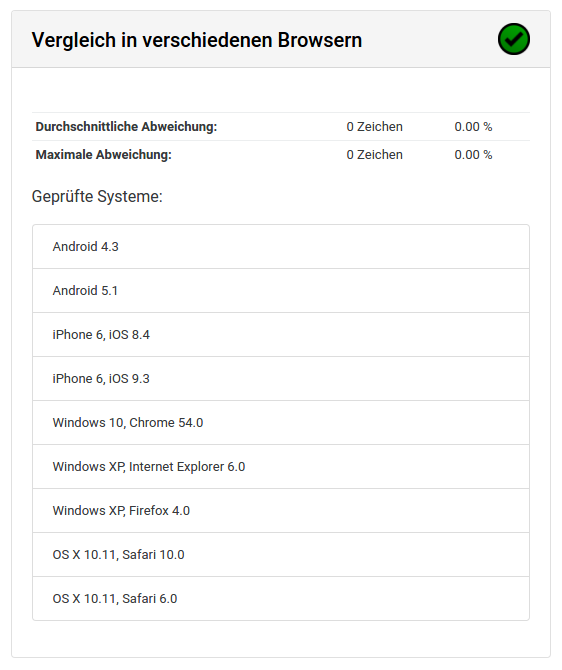
\includegraphics[width=0.5\textwidth]{images/platform/header-inspection-clean}%
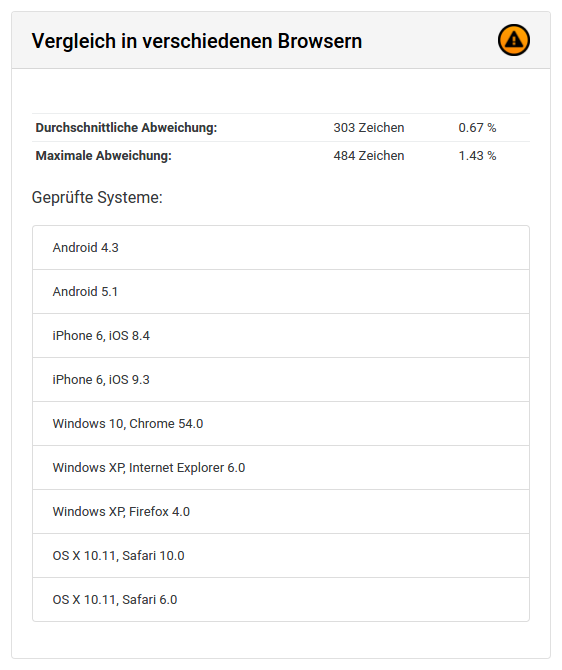
\includegraphics[width=0.5\textwidth]{images/platform/header-inspection-suspicious}%
}%
\caption{webifier Platform - Vergleich in verschiedenen Browsern}
\label{fig:platform-result-header-inspection}
\end{figure}

Der Vergleich in verschiedenen Browsern zeigt die maximale und die durchschnittliche Abweichung, sowohl als absoluten, als auch als prozentualen Wert. Zusätzlich erhält der Nutzer eine Übersicht uber alle Systeme, welche getestet und miteinander verglichen wurden. Zwei Beispielergebnisse hierfür sind in Abbildung \ref{fig:platform-result-header-inspection} zu sehen.

\begin{figure}[H]
\centerline{%
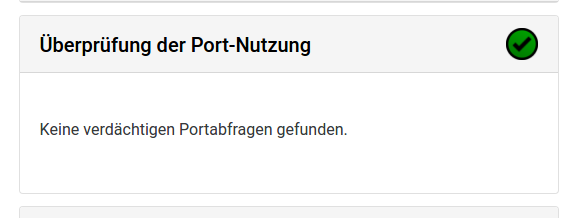
\includegraphics[width=0.5\textwidth]{images/platform/portscan-clean}%
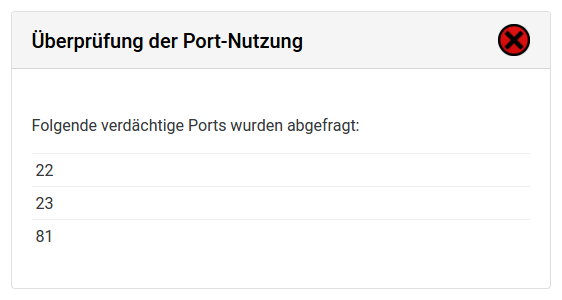
\includegraphics[width=0.5\textwidth]{images/platform/portscan-malicious}%
}%
\caption{webifier Platform - Überprüfung der Port-Nutzung}
\label{fig:platform-result-portscan}
\end{figure}

\begin{figure}[H]
  \centering
  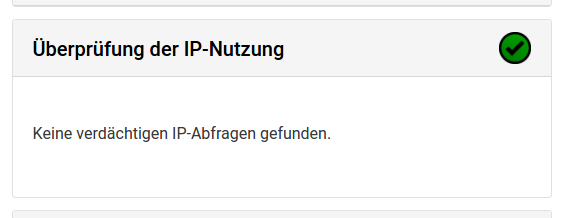
\includegraphics[width=7.5cm]{images/platform/ipscan-clean}
  \caption{webifier Platform - Überprüfung der IP-Nutzung}
  \label{fig:platform-result-ipscan}
\end{figure}

Abbildung \ref{fig:platform-result-portscan} zeigt die Ergebnisse der Überprüfung der Port-Nutzung, welche im Falle eines verdächtigen oder bedrohlichen Ergebnisses eine Liste mit allen gefundenen Ports enthält. Das Ergebnis der Überprüfung der IP-Nutzung ist gleich aufgebaut und in Abbildung \ref{fig:platform-result-ipscan} abgebildet. Es stellt bei entsprechenden Funden eine Liste aller IP-Adressen bereit.

\begin{figure}[H]
  \centering
  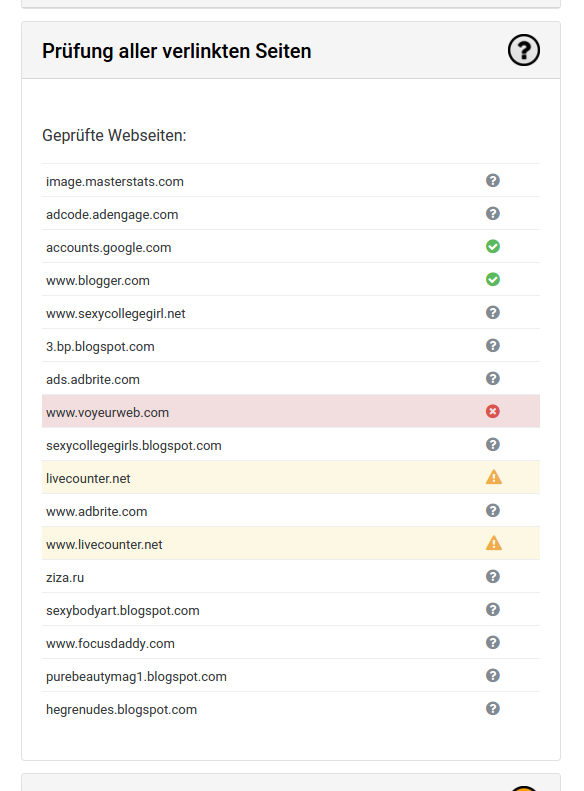
\includegraphics[width=7.5cm]{images/platform/linkchecker-undefined}
  \caption{webifier Platform - Prüfung aller verlinkten Seiten}
  \label{fig:platform-result-linkchecker}
\end{figure}

Das Ergebnis der Prüfung aller verlinkten Seiten enthält eine einfache Liste mit allen gefundenen Links und dem entsprechenden Ergebnis aus webifier Data. Abbildung \ref{fig:platform-result-linkchecker} zeigt eine solche Liste.

\begin{figure}[H]
\centerline{%
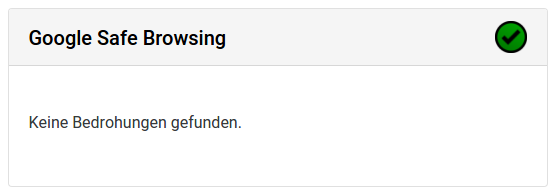
\includegraphics[width=0.5\textwidth]{images/platform/google-safe-browsing-clean}%
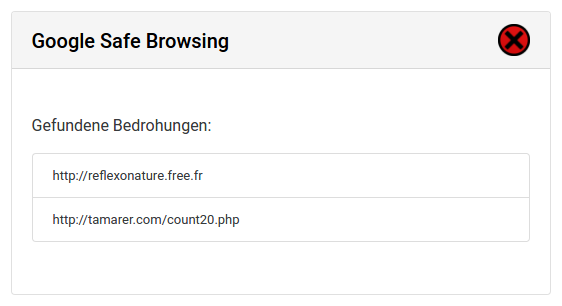
\includegraphics[width=0.5\textwidth]{images/platform/google-safe-browsing-malicious}%
}%
\caption{webifier Platform - Google Safe Browsing}
\label{fig:platform-result-google-safe-browsing}
\end{figure}

Die Deteilansicht des Google Safe Browsing Ergebnisses ist ähnlich dem der Prüfung aller verlinkten Seiten. Allerdings listet diese nur alle gefundenen Bedrohungen auf und nicht alle geprüften Links. Abbildung \ref{fig:platform-result-google-safe-browsing} enthält zwei Beispielresultate.

\begin{figure}[H]
\centerline{%
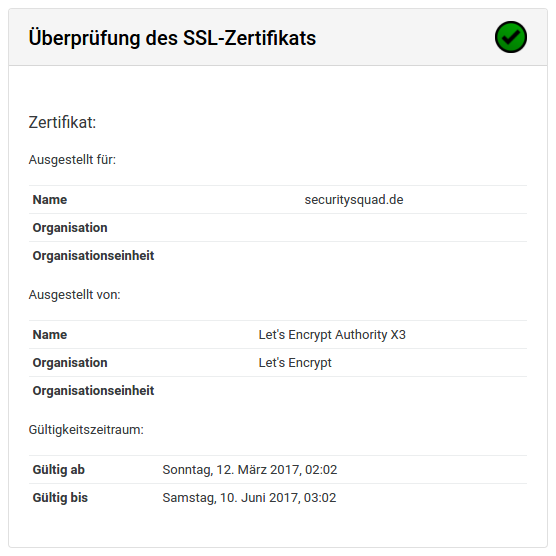
\includegraphics[width=0.5\textwidth]{images/platform/certificatechecker-clean}%
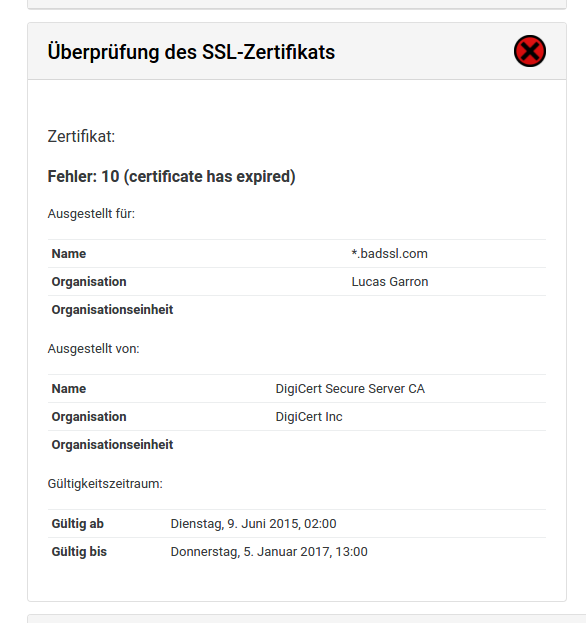
\includegraphics[width=0.5\textwidth]{images/platform/certificatechecker-malicious}%
}%
\caption{webifier Platform - Überprüfung des SSL-Zertifikats}
\label{fig:platform-result-certificatechecker}
\end{figure}

Das Ergebnis der Überprüfung des SSL-Zertifikates enthält alle Informationen des Zertifikats, sofern die Webseite eines nutzt. Wie in Abbildung \ref{fig:platform-result-certificatechecker} dargestellt, zeigt die Detailansicht einmal für wen das Zertifikat ausgestellt wurde, aber auch wer es ausgestellt hat. Außerdem wird der Gültigkeitszeitraum des Zertifikats angezeigt und im Fehlerfall der gefundene Fehler.

\begin{figure}[H]
\centerline{%
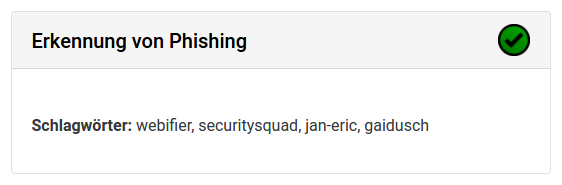
\includegraphics[width=0.5\textwidth]{images/platform/phishing-clean}%
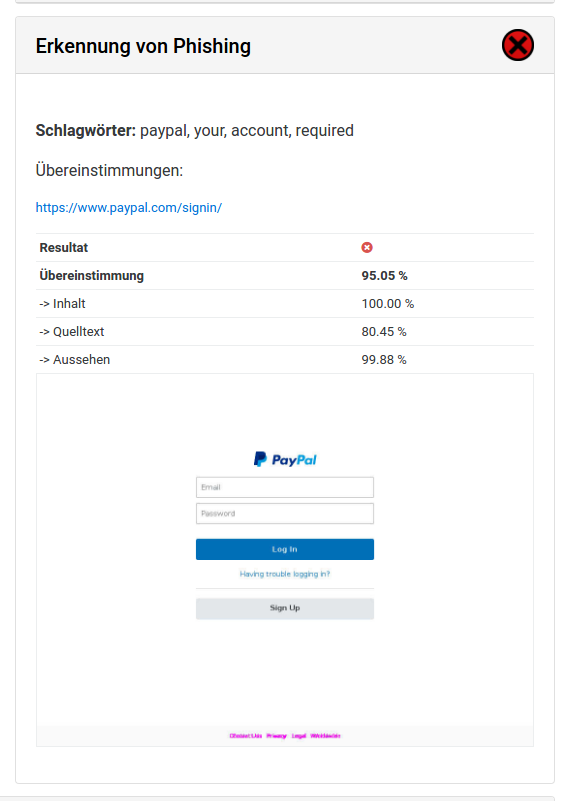
\includegraphics[width=0.5\textwidth]{images/platform/phishing-malicious}%
}%
\caption{webifier Platform - Erkennung von Phishing}
\label{fig:platform-result-phishingdetector}
\end{figure}

Die Erkennung von Phishing stellt ebenfalls einige Informationen zur Verfügung, wie Abbildung \ref{fig:platform-result-phishingdetector} zeigt. Es werden in jedem Fall die gefundenen Schlagwörter der Webseite angezeigt. Ist das Ergebnis verdächtig oder bedrohlich, so wird die vermeindliche Originalseite verlinkt, die Werte der prozentualen Übereinstimmungen insgesamt und von Inhalt, Quelltext und Aussehen separat aufgelistst und ein Bild der beiden überlagerten Seiten gezeigt. Alle Inhalte, welche sich unterscheiden werden rosa dargestellt. Im Beispiel aus der Abbildung unterscheidet sich demnach nur der Text der Fußzeile.

\begin{figure}[H]
  \centering
  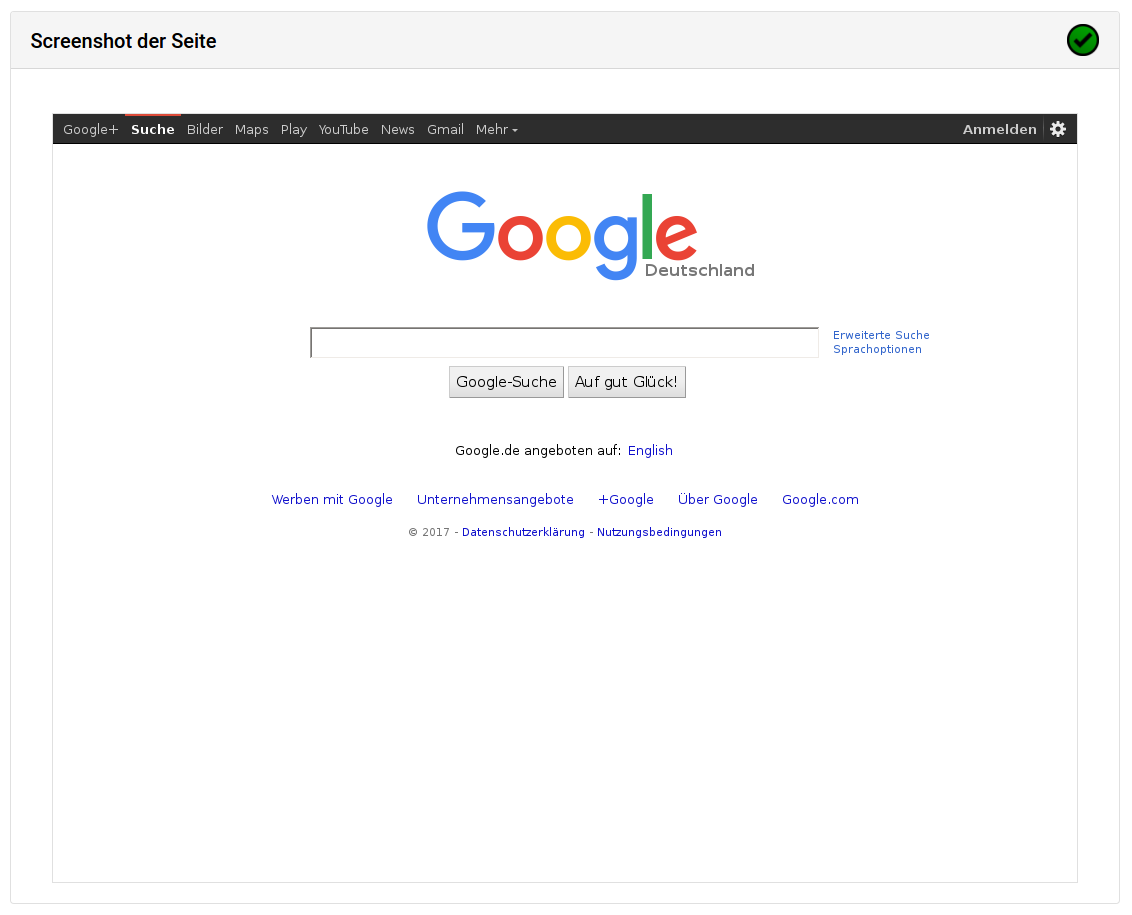
\includegraphics[width=\textwidth]{images/platform/screenshot-clean}
  \caption{webifier Platform - Screenshot der Seite}
  \label{fig:platform-result-screenshot}
\end{figure}

Der Screnenshot der Seite wird beim ausklappen des Panels einfach angezeigt, so wie es in Abbildung \ref{fig:platform-result-screenshot} dargestellt. Dies gibt dem Nutzer die Möglichkeit sich die Webseite anzusehen, ohne sie selbst zu besuchen.

Wie nun gezeigt bietet die Plattform seh viele interessante Zusatzinformationen zu den Testergebnissen, mit denen das Gesamtresultat noch genauer erklärt wird. Außerdem bekommt der Nutzer so genügend Informationen um die Plausibilität der Testergebnisse selbst noch einmal zu überprüfen.

\subsection{webifier Mail}

\todo{Daniel}

\subsection{webifier Data}
\label{sec:umsetzung-data}

webifier Data stellt eine Schnittstelle zur globalen Datenspeicherung der Testresultate zur Verfügung. Die Komponente setzt ebenfalls auf dem Spring-Framework auf und wurde deshalb in Java implementiert. Außerdem wird die Spring-Bibliothek Spring-Data eingesetzt um Java-Objekte auf Dokumente zu übertragen und in einer MongoDB zu persistieren.

Das Modul bietet eine \ac{REST}-\ac{API} zur externen Nutzung, beispielsweise im webifier Tester oder in der Prüfung aller verlinkten Seiten. Die API stellt die folgenden Aktionen bereit: \lstinline[style=eclipse]{/push}, \lstinline[style=eclipse]{/check} und \lstinline[style=eclipse]{/count}. Mit der Methode \lstinline[style=eclipse]{/push} können Testergebnisse in webifier Data abgelegt werden. Die entsprechende Resource, welche im Inhalt des POST-Requests gesendet werden muss ist in Listing \ref{lst:data-push} dargestellt.

\begin{scriptsize}
\lstset{
    style=eclipsejavascript,
    caption={Ausschnitt Inhalt push-Request - webifier Data},
    label={lst:data-push}
}
\begin{lstlisting}
{
    "id" : "33e76954-dc94-48a9-a816-99ddeb647887",
    "enteredUrl" : "securitysquad.de",
    "testedUrl" : "https://www.securitysquad.de/",
    "result" : {
        "resultType" : "CLEAN",
        "resultValue" : 0
    }
    "duration" : 46220,
    "testResults" : [
        {
            "testId" : "33e76954-dc94-48a9-a816-99ddeb647887_07bb1b72-fd9f-4286-ade5-2d71cf47580a",
            "testData" : {
                "name" : "VirusScan",
                "startup" : "docker run --rm --name #ID -e URL=#URL -e ID=#ID webifier-test-virusscan",
                "shutdown" : "docker stop #ID",
                "enabled" : true,
                "weight" : 5,
                "startupTimeoutInSeconds" : 600,
                "shutdownTimeoutInSeconds" : 30,
            },
            "result" : {
                "result" : "CLEAN",
                "resultInfo" : {
                    ...
                }
            },
            "duration" : 31191
        },
        ...
    ]
}
\end{lstlisting}
\end{scriptsize}

Die Methode \lstinline[style=eclipse]{/check} bietet die Möglichkeit webifier Data nach einer oder mehreren Urls zu durchsuchen. Hierfür muss im Inhalt des POST-Requests die in Listing \ref{lst:data-check-request} gezeigte Ressource gesendet werden. Diese enthält eine Liste der zu überprüfenden Links.

\begin{scriptsize}
\lstset{
    style=eclipsejavascript,
    caption={Inhalt check-Request - webifier Data},
    label={lst:data-check-request}
}
\begin{lstlisting}
{
    "urls": [
        "https://fonts.googleapis.com/css?family=Montserrat:400,700",
        "https://fonts.googleapis.com/css?family=Lato:400,700,400italic,700italic",
        "https://www.google.com/recaptcha/api.js",
        "https://cdnjs.cloudflare.com/ajax/libs/jquery-easing/1.3/jquery.easing.min.js",
        "https://www.gstatic.com/recaptcha/api2/r20170503135251/recaptcha__de.js",
        "https://fonts.gstatic.com/s/lato/v13/v0SdcGFAl2aezM9Vq_aFTQ.ttf",
        "https://fonts.gstatic.com/s/lato/v13/DvlFBScY1r-FMtZSYIYoYw.ttf",
        "https://www.gstatic.com/recaptcha/api2/r20170503135251/fallback__ltr.css",
        "https://fonts.googleapis.com/css?family=Roboto:400,500",
        "https://www.gstatic.com/recaptcha/api2/logo_48.png",
        "https://github.com/SecuritySquad",
        "https://www.webifier.de/",
        "https://github.com/SecuritySquad/webifier-platform",
        "http://djbrown.de/",
        "https://www.facebook.com/danjoebro",
        "https://github.com/djbrown",
        "https://plus.google.com/114056971447496286521",
        "https://github.com/jockelmore",
        "https://samuel-philipp.de/",
        "https://github.com/samuel-p",
        "https://plus.google.com/u/0/+SamuelPd"
    ]
}
\end{lstlisting}
\end{scriptsize}

Wie Listing \ref{lst:data-check} zeigt gruppiert webifier Data zunächst alle Links anhand deren Host-Teil und entfernt alle ungültigen Einträge. Anschließend werden alle Resultate für jeden Eintrag der Liste geladen und daraus ein Gesamtergebnis pro Host berechnet. Dieses wird schließlich mit dem Host als schlüssel zur Liste \textit{hostResults} hinzugefügt. Abschließend wird die erzeugte Liste als Ergebnis zurückgegeben und als Antwort zurückgesendet. Diese Antwort ist in Listing \ref{lst:data-check-response} abgebildet.

\begin{scriptsize}
\lstset{
    style=eclipsejava,
    caption={Verarbeitung check Methode - webifier Data},
    label={lst:data-check}
}
\begin{lstlisting}
$$@Override$$
public WebifierCheckTestResultsResponse checkTestResultsRequest(WebifierCheckTestResultsRequest request) {
    List<String> hosts = request.getUrls().stream().map(url -> {
        try {
            return filterHost(url);
        } catch (MalformedURLException e) {
            return null;
        }
    }).distinct().filter(StringUtils::isNotEmpty).collect(toList());
    Map<String, WebifierTestResultDetails> hostResults = new HashMap<>();
    hosts.forEach(host -> {
        List<WebifierTestResultData> data = #dataPersistenceService#.getTestResultDataByHost(host)
                .stream().filter(d -> d.getOverallResultType() != WebifierTestResult.##UNDEFINED##).collect(toList());
        if (data.isEmpty()) {
            hostResults.put(host, WebifierTestResultDetails.##UNDEFINED##);
        } else {
            double resultValue = data.stream().mapToDouble(this::mapDataResultToIndex).average().orElse(1);
            hostResults.put(host, mapResultValueToResult(resultValue));
        }
    });
    if (hostResults.isEmpty()) {
        return new WebifierCheckTestResultsResponse(false);
    }
    return new WebifierCheckTestResultsResponse(true, hostResults);
}
\end{lstlisting}
\end{scriptsize}

\begin{scriptsize}
\lstset{
    style=eclipsejavascript,
    caption={Inhalt check-Response - webifier Data},
    label={lst:data-check-response}
}
\begin{lstlisting}
{
    "success": true,
    "hosts": {
        "www.facebook.com": "CLEAN",
        "fonts.googleapis.com": "UNDEFINED",
        "plus.google.com": "CLEAN",
        "fonts.gstatic.com": "UNDEFINED",
        "cdnjs.cloudflare.com": "UNDEFINED",
        "github.com": "CLEAN",
        "djbrown.de": "UNDEFINED",
        "samuel-philipp.de": "UNDEFINED",
        "www.google.com": "SUSPICIOUS",
        "www.gstatic.com": "UNDEFINED",
        "www.webifier.de": "CLEAN"
    }
}
\end{lstlisting}
\end{scriptsize}

Die Methode \lstinline[style=eclipse]{/count} liefert einfach die aktuelle Gesamtzahl der in webifier Data vorhandenen Testergebnisse.

Die Testergebnisse werden in der MongoDB auf zwei Dokumente verteilt. Das erste Dokument (\lstinline[style=eclipse]{webifierTestResultData}) enthält alle Gesamtdaten des Resultats, das zweite (\lstinline[style=eclipse]{webifierSingleTestResultData}) umfasst alle Einzelergebnisse des Resultats. Deshalb werden pro Testergebnis ein Dokument in \lstinline[style=eclipse]{webifierTestResultData} und acht in \lstinline[style=eclipse]{webifierSingleTestResultData} gespeichert.

Zur Persistierung werden alle Informationen der \lstinline[style=eclipse]{/push} Methode (Listing \ref{lst:data-push}) auf die entspechenden Dokumente gemappt. Listing \ref{lst:data-resultdata} zeigt die transformierten Daten aus \lstinline[style=eclipse]{webifierTestResultData}. Anhang \appref{e} enthält die transformierten Dokumente aller Einzelergebnisse in \lstinline[style=eclipse]{webifierSingleTestResultData}.

\begin{scriptsize}
\lstset{
    style=eclipsejavascript,
    caption={Beispieldokument webifierTestResultData - webifier Data},
    label={lst:data-resultdata}
}
\begin{lstlisting}
{
	"_id" : "d62e8c94-21c9-4d69-9337-186b38f73cce",
	"_class" : "de.securitysquad.webifier.persistence.domain.WebifierTestResultData",
	"testerId" : "56821bd8-f652-4b59-b7ec-12faa7cf6cae",
	"enteredUrl" : "ukauctionline.co.uk",
	"testedUrl" : "http://ukauctionline.co.uk",
	"host" : "ukauctionline.co.uk",
	"overallResultType" : "SUSPICIOUS",
	"overallResultValue" : 0.057291666666666664,
	"durationInMillis" : NumberLong(227639),
	"datetime" : ISODate("2017-03-28T22:32:53.834Z"),
	"testResults" : [
		DBRef("webifierSingleTestResultData", "5ecb25e6-457b-41ab-9241-a60f8a484131"),
		DBRef("webifierSingleTestResultData", "abb70569-64d3-47ae-b3e3-ff8086c8f937"),
		DBRef("webifierSingleTestResultData", "56dbbcb3-9628-4dd4-bb20-692bd86c5410"),
		DBRef("webifierSingleTestResultData", "64ae09d4-a79e-4194-b77c-3a7891342567"),
		DBRef("webifierSingleTestResultData", "05ba8488-4b69-40f9-8a9d-661c09daab65"),
		DBRef("webifierSingleTestResultData", "e0ce8955-feb7-4f7a-adfb-b7b8116a9d28"),
		DBRef("webifierSingleTestResultData", "9affd5e9-37eb-4d83-b471-ceab0c19155c"),
		DBRef("webifierSingleTestResultData", "c2b02bf9-2073-451b-a566-295fe1801e51")
	]
}
\end{lstlisting}
\end{scriptsize}

\subsection{webifier Statistics}
\label{sec:umsetzung-statistics}

Webifier Statistics wird in R implementiert. Hierzu werden Flexdashboards\footnote{\url{http://rmarkdown.rstudio.com/flexdashboard/index.html}} verwendet. Zur Generierung der Grafiken wurde auf verschiedene Librarys, wie beispielsweise Plot.ly, zurückgegriffen um den Entwicklungsaufwand für die Visualisierungen zu minimieren. Die Anordnung der Grafiken wird über ein bestimmtes Layout definiert. Jede Grafik wird prinzipiell in 3 Schritten erstellt:

\begin{enumerate}
  \item Daten aus der MongoDB laden
  \item Daten in die benötigte Form transformieren
  \item Entsprechende API ansteuern für Generierung der Grafik
\end{enumerate}

\begin{scriptsize}
\lstset{
    style=eclipsejavascript,
    caption={Beispiel R-Grafik},
    label={lst:rgrafik}
}
\begin{lstlisting}
  ### Durchschnittliche Analysezeit

  ```{r}
  result <- dbGetQueryForKeys(mg1, 'webifierTestResultData',"{}", "{durationInMillis:1}",skip=0,limit=Inf)
  mean.dur <- mean(result$durationInMillis)/1000
  mean.dur <- round(mean.dur)
  tp <- seconds_to_period(mean.dur)
  valueBox(paste(minute(tp),'min ',second(tp),'s',sep=""), icon="fa-hourglass-half",color="grey")
  ```
\end{lstlisting}
\end{scriptsize}

Im Codebeispiel \ref{lst:rgrafik} ist der Codeablauf für eine Valuebox zu sehen. Dieses Beispiel wurde ausgewählt um den Erstellungsprozess für die Grafiken zu erklären. Dies lässt sich auf alle anderen Grafiken übertragen.

Die Überschriften der Grafiken werden mit \textit{\#\#\#} markiert. Der R-Code befindet sich in Chunks, diese werden speziell markiert um dem Compiler kenntlich zu machen welches der R-Code ist.

Im Beispiel werden zunächst benötigten Daten aus der MongoDB geladen. Da hier eine Valuebox für die Anzeige der durchschnittlichen Analysezeit generiert wird werden nur die Analysezeiten(durationInMillis) benötigt. Diese werden anschließend gemittelt und von Millisekunden in Minuten/Sekunden transformiert. Zur Erstellung der Valuebox muss nun nurnoch der Text, die Farbe und ein passendes Icon ausgewählt werden. Die Generierung und Platzierung übernimmt Flexdashboard. Als Ausgabe wird eine HTML-Datei generiert, welche dann in den Webserver eingebunden wird um sie für die Nutzer zugänglich zu machen.

\begin{figure}[H]
  \centering
  
\includegraphics[width=5cm]{images/stats/valuebox}
  \caption{Generierte Valuebox}
  \label{fig:valuebox}
\end{figure}

In Abbildung \ref{fig:valuebox} ist die fertig generierte Valuebox mit Überschrift, Text und Icon in passender Farbe dargestellt.

Für stets aktuelle Grafiken wird das R-Skript für die Statistiken mehrfach täglich neu gebaut um die aktuellen Daten mit einzubeziehen. Von einer \textit{On the fly}-Generierung der Grafiken wurde abgesehen, da dies für den Server zu rechenintensiv wäre.

\section{Tests}

In diesem Abschnitt werden nun die Implementierungen aller Einzeltests erklärt. Bei allen kam zur Isolierung die Technologier Docker zum Einsatz.

\subsection{Virenscan der Webseite}

Der Virenscan der Webseite wurde in Python umgesetzt und lädt zunächst alle Ressourcen der Webseite in ein lokales Verzeichnis herunter. Hierbei kommt die Software HTTrack zum Einsatz. HTTtrack wird für diesen Zweck speziell konfiguriert, um die Antwortzeiten so gering wie möglich zu halten. Zunächst wird der Downloadmodus so gewählt, dass einfach nur alle Dateien gespeichert werden, ohne sie für die dauerhafte Nutzung bereitzuhalten. Des weiteren darf keine Datei im Inhalt verändert werden, da so das Ergebnis verfälscht werden könnte. Um zeit zu spaaren wird zusätzlich auf die protokollierung verzichtet. Außerdem sollen die \lstinline[style=eclipse]{robots.txt} Dateien ignoriert werden, da damit Malware auch vor Suchmaschinen versteckt werden kann. Schießlich wird HTTrack eine maximale Laufzeit zum Download aller Dateien von drei Minuten gewährt.

Zum Scannen aller gespeicherten Dateien kommen drei Virenscanner zum Einsatz. Es werden die Antivirenprogramme ClamAV\footnote{\url{http://www.clamav.net/}}, AVG\footnote{\url{http://www.avg.com/de-de/homepage}} und Comodo Antivirus\footnote{\url{https://antivirus.comodo.com/}} verwendet. Um auch hier die Antwortzeiten gering zu halten werden die Virenscannner parallel ausgeführt.

Abschließend werden alle Ergebnisse der Antivirenprogramme ausgewertet und daraus das Gesamtergebnis gebildet. Dieses wird inklusive der Liste aller bewertetetn Dateien weitergeleitet.

\subsection{Vergleich in verschiedenen Browsern}

Dieser Test wird durch zwei Schritte ermöglicht.
Zunächst werden für eine Liste von Browserkonfigurationen deren \ac{HTTP}-Header ermittelt, danach werden Requests mit diesen Headern an die zu testende \ac{URL} geschickt und die Antworten untereinander verglichen.
Damit nicht bei jedem Testdurchlauf alle Header neu eingeholt werden müssen, werden sie in einer Datei abgespeichert.

Zur Umsetzung dieses Tests wurde zunächst ein Python-Skript geschrieben, welches über einen Cloud-Service die Werte für das \ac{HTTP}-Headerfeld \textit{User Agent} abspeichert.
Zuerst werden alle gewünschten Browserkonfigurationen über eine \ac{JSON}-Datei eingelesen (s. Zeile 31).
Diese Datei enthält eine Liste von Browserobjekten, die die Konfigurationen im Attribut 
Ein Element dieser Liste ist beispielhaft in \autoref{lst:browsers.json} zu sehen, wobei das \lstinline{"headers"}-Attribut vor Programmablauf noch nicht gesetzt ist.

\begin{scriptsize}
\lstset{
	style=eclipsejavascript,
	caption={Beispiel für Browserkonfiguration und gespeicherte Header},
	label={lst:browsers.json}
}
\begin{lstlisting}
[{"configuration": {
    "platform": "Windows XP",
    "browserName": "internet explorer",
    "version": "6.0",
    "name": "Windows XP, Internet Explorer 6.0"
  },
  "headers": {
    "Host": "www.reliply.org",
    "Request Method": "GET",
    "User Agent": "Mozilla/4.0 (compatible; MSIE 6.0; Windows NT 5.2; SV1; .NET CLR 1.1.432)",
    "Accept Encoding": "gzip, deflate",
    "Accept Language": "en-us",
    "HTTP Connection": "keep-alive"
}}]
\end{lstlisting}
\end{scriptsize}

Danach werden für jeder dieser Konfigurationen die entsprechenden Header ermittelt.
Dazu wird eine Verbindung mittels \ac{SSH} zum Service \textit{Sauce Labs} aufgebaut.
Dabei wird auch ein ferngesteuerter Browser mit der Konfiguration des lokalen Browserobjekts initialisiert.
Das Browserobjekt ist wie ein Headless Browser über das Modul \textit{WebDriver} steuerbar.
Im nächsten Schritt wird der Browser dann angewiesen auf die Webseite \url{http://www.reliply.org/tools/requestheaders.php} zu gehen.
Auf dieser Seite werden alle \ac{HTTP}-Headerfelder und deren Werte in einer Tabelle aufgelistet.
Ein Beispiel dafür ist in \autoref{fig:reliply} zu sehen.
Diese Tabelle beinhaltet in der ersten Spalte den Headernamen und in der zweiten den Wert.
Diese beiden Daten werden in jeder Zeile der Tabelle 
Der Brower greift auf diese beiden Daten in jeder Zeile der Tabelle zu und speichert diese im Browserobjekt.
Es werden alle Header bis auf den \lstinline{Host}-Header abgespeichert, da dieser lediglich der Domain des Zielserver entspricht.
Nachdem alle Header zu den Browserkonfigurationen heruntergeladen wurden, wird die Liste der Browserobjekte in die Datei \lstinline{browser.json} abgespeichert.

\begin{figure}[H]
	\centering
	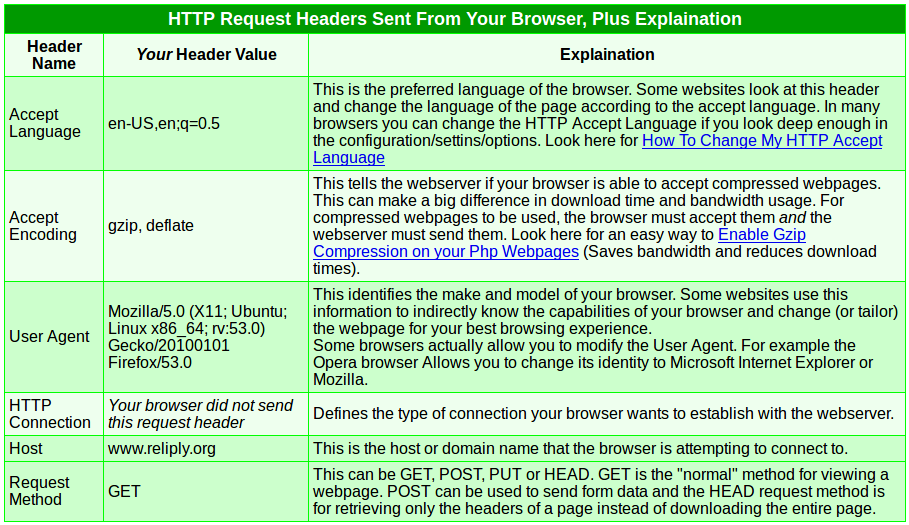
\includegraphics[width=\textwidth]{images/reliply.png}
	\caption{Tabelle der \ac{HTTP}-Header auf \url{reliply.org}}
	\label{fig:reliply}
\end{figure}

Ursprünglich basierte die Berechnung der Abweichungen auf Prozentwerten.
Während der Implementierung ist aufgefallen, dass die prozentualen Abweichungen der Antworten keine zuverlässige Auskunft über einen möglichen Angriff auf den Nutzer geben können.
Aus diesem Grund wird die Ergebniskalkulation nun auf absoluten Abweichungswerten ausgeführt.
Dabei wird jede Browserantwort jeweils einmal mit jeder anderen verglichen und der niedrigste absolute Übereinstimmungswert, 
überprüft werden, ob der schlechteste Wert unter einer bestimmten Grenze liegt, da er sonst statistisch untergehen würde.
\todo{fertig schreiben}


\subsection{Überprüfung der Port-Nutzung}
Bei diesem Test wird überprüft ob die Seite versucht einen Portscan auf dem Computer des Anwenders zu betreiben. Hierfür werden 3 Techniken eingesetzt. Die wichtigsten Aufgaben werden von PhantomJS und Bro erledigt.
Bro ist ein Netzwerkmonitoringtool und wird hier genutzt um den Traffic welcher zwischen Webseite und Client entsteht zu protokollieren und in einer Logdatei abzuspeichern. PhantomJS ist ein \textit{headless Browser}, welcher genutzt wird um die Webseite aufzurufen und dessen Javascript auszuführen. Das ganze funktioniert hier ohne grafische Oberfläche.

Der Ablauf des Tests sieht wie folgt aus: Zunächst wird Bro intialisiert und es werden Filter angelegt um lediglich die Ports, der eingehenden Anfragen, mitzuloggen und in der Logdatei abzuspeichern. Ist Bro vollständig initialisiert und einsatzbereit startet PhantomJS mit dem Aufrufen der Seite und Ausführen des JavaScript-Codes. Währenddessen speichert Bro alle Netzwerkaktivitäten. Sobald der Durchlauf von PhantomJS abgeschlossen ist wird mittels Python die Validierung des Ergebnisses gestartet. Hier werden die angefragten Ports aus der Logdatei geladen und klassifiziert. Die Ports 80 und 443 werden verworfen, da diese die HTTP und SSL Ports sind und somit als harmlos klassifiziert werden können. Die weiteren Ports werden in einer Liste an riskanten Ports gespeichert. Die Anzahl an Ports in dieser Liste bestimmt nun das Ergebnis des Testes. Wurden keine verdächtigen Portanfragen gefunden wird das Ergebnis \textit{unbedenklich} übermittelt. Bei 1 oder 2 Ports in der Liste gibt der Test \textit{verdächtig} als Ergebnis zurück. Sollte die Anzahl größer gleich 3 sein wird die Seite von diesem Test als \textit{bedrohlich} eingestuft. Zusätzlich zum Ergebnis wird die Liste der riskanten Ports in der Ergebnisinformation weitergeleitet.

\subsection{Überprüfung der IP-Nutzung}
Der Test auf verdächtige IP-Anfragen ist bis auf 2 Änderungen identisch zu vorherigem Test auf Portscanning. Deshalb werden in diesem Kapitel nur die Unterschiede beleuchtet.

Der erste Unterschied liegt in der Initialisierung von Bro. Hier werden Filter angewendet um die IPs, der ausgehenden Anfragen, zu loggen. Hier müssen die ausgehenden Anfragen betrachtet werden, da bei dieser Art von Angriff versucht wird mittels clientseitig ausgeführtem JavaScript das Netzwerk des Anwenders auszuspähen. Den Aufruf der Seite übernimmt auch hier PhantomJS. Bei der darauf folgenden Validierung werden die IPs auf bekannte Heimnetzadressbereiche wie beispielsweise 192.168.178.* oder 192.168.2.* gemappt. Auch hier werden verdächtige IPs in einer Liste gespeichert. Die Anzahl der Elemente in dieser Liste bestimmt das Ergebnis des Testes. Hierbei sind die Schwellwerte identisch mit denen des Portscanning-Tests, also bei 0 Abfragen wird \textit{sauber} zurückgegeben, bei 1-2 wird \textit{verdächtig} zurückgegeben und bei >3 wird die Seite als \textit{bedrohlich} eingestuft. Zusätzlich zum Ergebnis wird die Liste der riskanten IPs in der Ergebnisinformation weitergeleitet.

\subsection{Prüfung aller verlinkten Seiten}

Dies wird über das Framework \textit{PhantomJS} bewerkstelligt, das in \autoref{par:phantomjs} vorgestellt wurde.
Dazu werden -Requests \ac{REST}-\ac{API}

\subsection{Google Safe Browsing}

\todo{Daniel}

\subsection{Überprüfung des SSL-Zertifikats}

Der Test zur Überprüfung des SSL-Zertifikates wurde mit Python und in Docker umgesetzt. Technisch wurde zur Überprüfung auf die \ac{CLI}-Anwendung \textit{openssl} gesetzt. Mit dieser wurden alle verfügbaren Informationen des Zertifikats der Webseite ausgelesen und zwischengespeichert.

Anschließend wurden alle Daten zusammengetragen und daraus das entsprechende Endergebnis erzeugt. Nutzt die Webseite kein Zertifikat, so ist das Ergebnis \textit{SUSPLCIOUS}. Hat die Webseite ein gültiges Zertifikat, dann ist das Ergebnis des Tests \textit{CLEAN}. Nutzt die Webseite ein fehlerhaftes Zertifikat, so wird das Ergebnis \textit{MALICIOUS} zurückgegeben. Tritt während dem Test ein unbekannter Fehler auf, so endet der Test mit dem Ergebnis \textit{UNDEFINED}. Zusätzlich zum Ergebnis werden alle ausgelesenen Informationen des Zertifikats an den Tester zurückgegeben.

\subsection{Erkennung von Phishing}
\label{sec:umsetzung-phishungdetector}

Die Erkennung von Phishing kann sehr komplex und umfassend werden. Deshalb wurde der Phishing Detector für diese Arbeit sehr einfach gehalten und beschränkt sich auf eine Grundlagenuntersuchung. Der Test umfasst sieben Teilschritte, welche nun genauer erläutert werden.

Im ersten Schritt wird die gegebene Webseite mit Hilfe von PhantomJS aufgerufen und ausgewertet. Diese Auswertung umfasst die gefundenen Schlüsselwörter der Seite, welche im nächsten Schritt zum Finden möglicher Originale benötigt werden. Außerdem wird ein Screenshot von der Webseite gespeichert, der Quelltext ausgelesen und auf die zum Inhalt gehörenden Wörter reduziert. Zusätzlich wird untersucht, ob die Seite Passworteingabefelder enthält. All diese Informationen gibt PhantomJS an das Python-Skript zurück.

Wenn mindestens ein Schlüsselwort gefunden wurde folgt nun der nächste Schritt. Wurde kein Schlüsselwort gefunden, so endet der Test mit dem Ergebnis \textit{UNDEFINED}. Der zweite Schritt ist das Finden von Links für mögliche Originale der zu überprüfenden Seite. Hierfür wird einmal das erste Schlüsselwort verwendet um eine mögliche Domain daraus zu bilden. Für die Domainbildung werden die 5 meist genutzten Domainendungen\footnote{\url{https://w3techs.com/technologies/overview/top_level_domain/all}} (.com, .ru, .net, .org und .de) eingesetzt. Außerdem werden alle gefundenen Schlagwörter genutzt um in verschiedene Suchmaschinen danach zu suchen und so Links zu möglichen Dupplikaten zu finden. Zur Suche werden die drei Suchmaschinen DuckDuckGo\footnote{\url{https://duckduckgo.com/}}, Ixquick\footnote{\url{https://www.ixquick.com/}} und Bing\footnote{\url{https://www.bing.com/}} verwendet. Von jeder Suchmaschine werden die ersten zehn Eintrage weiterverarbeitet und in einer Gesamtliste mit den erzegten Domains zusammengeführt. Links die in mehreren Suchmaschinen aufgelistet werden steigen im Ranking auf. Am Ende dieses Schrittes wird die Liste auf 25 Eintrage reduziert.

Im nächsten Schritt müssen nun die Originalseiten herausgefiltert und aus der Liste der möglichen Originale entfernt werden, da viele Webseiten, beispielsweise die von Google unter vielen unterschiedlichen Domains erreichbar ist. Um dies zu erreichen wurden mehrere Methoden angewandt. Als erstes werden alle Links aufgelöst, um tatsächlich den Link der zu vergleichenden Seite zu nutzen. Ist der Link nicht erreichbar, oder führt er ins Nichts, so wird er aussortiert. Anschließend wird die Url auf die registrierte \ac{TLD} reduziert und mit der der gegebenen Seite verglichen. Beispielsweise wird \lstinline[style=eclipse]{https://abc.example.com/xyz} auf \lstinline[style=eclipse]{example.com} minimiert. Sind beide gleich, so wird der Link verworfen. So werden Unterseiten und Subdomains der gegeben Seite aussortiert. Als nächstes wird die IP-Adresse der Domain aufgelöst und mit der der zu prüfenden Seite verglichen. Sind diese identisch wird auch dieser Link aus der Liste entfernt. Als letztes werden die Zertifikatinformation der Links ausgelesen, sofern ein SSL-Zertifikat verfügbar ist. Anschließend werden die \textit{Subject}-Informationen des Zertifikates mit denen der gegebenen Seite verglichen. Sind diese gleich, so scheidet auch dieser Link aus. Nun wird die Liste der übrig gebliebenen Links noch auf zehn Links reduziert, welche nun im nächsten Schritt aufgerufen werden.

Der vierte Schritt ist das abrufen der Links der möglichen Originalwebseiten. Wie im ersten Schritt für die gegebene Seite werden nun für alle Links der Quelltextausgelesen, daraus der Inhalt extrahiert und ein Screenshot angefertigt. Alle hierbei gewonnenen Informationen werden im folgenden Schritt für den Vergleich benötigt.

Nun folgt der eigentliche Schritt des Vergleichens der möglichen Originale mit der zu validierenden Webseite. Der Vergleich erfolgt in den drei Bereichen Quelltext, Inhalt und Aussehen. Zum Quelltext- und Inhaltsvergleich werden Funktionen (\textit{difflib.SequenceMatcher(\ldots).quick\_ratio()}) der Python-Standardbibliothek verwendet. Für den Vergleich der Screenshots wurde auf die freie Bibliothek Resemble.js zurückgegriffen. Diese liefert für den Vergleich von zwei Bildern die prozentuale Übereinstimmung und erzeugt einen Differenzbild. All diese Daten wurden den Links zugeordnet und im nächsten Schritt zur Ergebnisberechnung verwendet.

Im vorletzten Schritt werden nun alle Links klassifiziert. Wie Listing \ref{lst:phishingdetector-result} werden zunächst werden die Schwellwerte der einzelnen Ergebnisklassen festgelegt. Diese sind davon abhängig, ob Passworteingabefelder auf der Seite vorhanden sind und ob die Seite ein SSL-Zertifikat nutzt. Besitzt die Seite mindestens ein Passwortfeld und nutzt kein Zertifikat, so werden die Schwellwerte um 0.05 reduziert. Anschließend wird die Durchschnittsübereinstimmung der beiden Seiten berechnet. In diese Rechnung fließt das Ergebnis des Screenshotvergleichs mit doppeltem Gewicht ein, da dieses am Aussagekräftigsten ist. Letztendlich werden die Links mit Hilfe der Schwellwerte und der berechneten Werte der Übereinstimmung klassifiziert. Hierfür gibt es einmal einen Mindestschwellwert für die Durchschnittsübereinstimmung, ab dem ein Ergebnis greift und Schwellwerte für die einzelnen Bereiche, in denen verglichen wurde. Die Bedingungen in den Zeilen 20 und 25 in Listing \ref{lst:phishingdetector-result} zeigen die Fälle, in denen ein Link \textit{SUSPICIOUS} oder \textit{MALICIOUS} ist.

\begin{scriptsize}
\lstset{
    style=eclipsepython,
    caption={Ergebnisberechnung der Erkennung von Phishing},
    label={lst:phishingdetector-result}
}
\begin{lstlisting}
def calculate_result(website, response):
    ratio_subtract = 0
    if website['password_field'] and not website['certificate']:
        ratio_subtract = 0.05

    suspicious_min = 0.82 - ratio_subtract
    suspicious_min_with_other = 0.77 - ratio_subtract
    suspicious_screenshot_min = 0.91 - ratio_subtract
    suspicious_html_min = 0.93 - ratio_subtract
    suspicious_content_min = 0.95 - ratio_subtract

    malicious_min = 0.9 - ratio_subtract
    malicious_min_with_other = 0.85 - ratio_subtract
    malicious_screenshot_min = 0.96 - ratio_subtract
    malicious_html_min = 0.97 - ratio_subtract
    malicious_content_min = 0.98 - ratio_subtract

    ratio = (response["screenshot_ratio"] * 2 + response["html_ratio"] + response["content_ratio"]) / 4
    result = "CLEAN"
    if ratio > suspicious_min or (ratio > suspicious_min_with_other
            and (response["screenshot_ratio"] > suspicious_screenshot_min
                or response["html_ratio"] > suspicious_html_min
                or response["content_ratio"] > suspicious_content_min)):
        result = "SUSPICIOUS"
    if ratio > malicious_min or (ratio > malicious_min_with_other
            and (response["screenshot_ratio"] > malicious_screenshot_min
                or response["html_ratio"] > malicious_html_min
                or response["content_ratio"] > malicious_content_min)):
        result = "MALICIOUS"
    return ratio, result
\end{lstlisting}
\end{scriptsize}

Der letzte Schritt berechnet abschließend das Endergebnis des Tests. Ist mindestens ein Link \textit{SUSPICIOUS} oder \textit{MALICIOUS}, so ist auch das Endergebnis entsprechend \textit{SUSPICIOUS} oder \textit{MALICIOUS}. Andernfalls ist das Gesamtergebnis des Tests \textit{CLEAN}.

\subsection{Screenshot der Seite}
Der Screenshot der Seite erfolgt über eine von PhantomJS gelieferte Methode um den Seiteninhalt aufzunehmen und als Bilddatei abzuspeichern. PhantomJS wird hierbei genutzt da der Test in einem Docker ohne grafische Benutzeroberfläche läuft und deshalb ein headless Browser nötig ist um die Seite aufzurufen. Nachdem die Seite in einer Bilddatei abgespeichert ist, wird diese als base64-encoded String weitergegeben. Der Test liefert immer das Ergebnis \textit{sauber}, welches aber für den Tester irrelevant ist, da der Screenshot-Test keine Gewichtung im Tester hat. In der Ergebnisinformation wird der base64 encodierte String weitergegeben, welcher dann von der Plattform interpretiert und als Bild für den Nutzer dargestellt wird.

\chapter{Analyse}

\begin{itemize}
  \item Daten
  \begin{itemize}
    \item Welche Listen wurden verwendet?
    \item Woher kommen die?
  \end{itemize}
  \item Statistische Auswertung
  \begin{itemize}
    \item Gesamtauswetungen
    \item Kleine Abschnitte für Einzelauswertungen der Tests
  \end{itemize}
  \item Disskusion
  \item Bewertung
\end{itemize}
\chapter{Ausblick}

Mit \textit{webifier} wurde eine modulare und leicht zu erweiternde Basis zur automatisierten Überprüfung
von Webseiten geschaffen. Der Umfang von \textit{webifier} kann in Zukunft durch zusätzliche Projekte
erweitert werden.

Der Umfang von \textit{webifier} kann sowohl in Form von neuen Tests zur Überprüfung weiterer clientseitigen
Angriffsszenarien, als auch in Form neuer Teilanwendungen, welche neue Funktionen für
die Endnutzer bereitstellen, erweitert werden. So kann die Bedrohlichkeit von Webseiten noch besser
klassifiziert werden und dem Nutzer können noch genauere Informationen zur Verfügung gestellt
werden.

Ein solches Modul könnte beispielsweise ein Browserplugin sein, welches automatisch vor dem Abrufen
einer Webseite \textit{webifier Data} nach Einträgen zu dieser Seite durchsucht und den Nutzer bei
Bedrohungen entsprechend warnt. Eine andere Möglichkeit wäre es die Analyse direkt über den Browser
anzustoßen, was allerdings gravierende Auswirkungen auf das Nutzerverhalten hätte, da die
Überprüfung einer Webseite etwa vier Minuten in Anspruch nimmt.

Des Weiteren können bereits implementierte Test noch erweitert und so das Gesamtergebnis der
Überprüfungen optimiert werden, da viele Tests noch sehr oberflächlich sind und alleine Potential
für mehrere Arbeiten liefern.

Außerdem kann durch weitere Überprüfungen von Websseiten der Datenbestand erweitert werden, was neue
Auswertungsmöglichkeiten für \textit{webifier Statistics} schafft. Mit größeren Datenmengen können
zuverlässiger statistische Zusammenhänge analysiert werden. Durch weitere Diagramme können neue
Erkenntnisse gewonnen werden.

Dies ließe sich beispielsweise durch eine neue Webcrawler-Erweiterung für \textit{webifier} realisieren. Diese würde dann alle externen Links einer Webseite extrahieren und automatisiert der Warteschlange hinzufügen. So könnten systematisch Informationen über ganze Bereiche des Internets gewonnen und ausgewertet werden.

\textit{webifier Plattform} und \textit{webifier Mail} könnten noch über einen gemeinsamen Scheduler abstrahiert
werden. Dieser könnte auch eine horizontale Skalierbarkeit der Überprüfung ermöglichen, welche
momentan noch nicht implementiert ist.

Des weiteren bietet das Darknet ein großes Potential um weitere Analysen zu starten. Hierfür
müsste ein neues Modul entwickelt werden welches die Webseiten abruft, da diese nicht über eine
normale Verbindung erreicht werden können.

Dank seiner Modularität bietet \textit{webifier} optimale Möglichkeiten für eine Weiterentwicklung.
\chapter{Fazit}

Die Motivation dieser Arbeit war es den Nutzern des Internets eine Möglichkeit zu bieten Webseiten
auf ihre Vertrauenswürdigkeit, bzw. ihre Bedrohlichkeit hin überprüfen zu lassen. Hierfür sollten
die Aktivitäten von Webseiten anhand verschiedener Tests analysiert und ausgewertet werden. Mit
\textit{webifier} wurde ein solches System geschaffen.

Bereits in der Konzeption wurden Modularität und einfache Erweiterbarkeit des Systems als Ziele
verfolgt. So wurde \textit{webifier} in seine Teilanwendungen gegliedert, welche über einheitliche
Schnittstellen miteinander kommununizieren. Dem Nutzer wurde die Interaktion über \textit{webifier Plattform} und
\textit{webifier Mail} ermöglicht.

Aus diesem Konzept folgte die Entwicklung der einzelnen Teilanwendungen. Diese wurden mit weit
verbreiteten Technolorien und Frameworks umgesetzt. Außerdem war es notwendig die Tests in einer
isolierten Umgebung auszuführen, um das eigene System vor Angriffen und möglichem Schaden zu
schützen.

Darauf folgend wurde eine großflächige Analyse von Webseiten durchgeführt, deren Ergebnisse in
\textit{webifier Data} gespeichert wurden. Anschließend nutzte \textit{webifier Statistics} diese Daten um
Auswertungen zu erstellen und diese für den Nutzer zu visualisieren. Bei diesen Diagrammen wurden
die gesammelten Daten genau betrachtet. In der Folge wurden die gewonnenen Erkenntnisse
untersucht und bewertet.

Abschließend lässt sich festhalten, das \textit{webifier} ein großes Potential und viele Möglichkeiten zur
Weiterentwicklung und Verwirklichung neuer Ideen geschaffen hat.

%Römische Nummerierung --> SeitenzahlSpeicher
\stepcounter{SeitenzahlSpeicher}
\renewcommand{\thepage}{\Roman{page}}
\setcounter{page}{\theSeitenzahlSpeicher}

%Anhang
\setlength\bibitemsep{12pt}
\printbibliography

%Anhang
\addchap{Anhang}

\section*{TEIL A: Autoren der einzelnen Kapitel}
Auf den folgenden Seiten werden die Kapitel in den Farben der Autoren markiert.
Dabei steht die Farbe blau für \daniel{Daniel Brown}, grün für \jani{Jan-Eric Gaidusch} und gelb für \samuel{Samuel Philipp}.

\rule{\textwidth}{1pt}

\daniel{Abstract}

{1 Einleitung}

\samuel{1.1 Einf\"uhrung}

\jani{1.2 Hintergrund}

\samuel{1.3 Aufgabenstellung}

\daniel{1.4 Team}

\samuel{1.5 webifier}

{2 Grundlagen}

\daniel{2.1 Frontend Technologien und Framework}

{2.2 Backend Technologien und Frameworks}

\indent \samuel{- Java}

\indent \samuel{- Spring}

\indent \samuel{- MongoDB}

\indent \jani{- Gradle}

\indent \jani{- Rest}

\indent \jani{- Docker}

\indent \jani{- R}

{2.3 Technologien und Frameworks der Tests}

\indent \daniel{- Python}

\indent \daniel{- PhantomJS}

\indent \jani{- Bro}

\indent \samuel{- HTtrack}

\indent \samuel{- Resemble.js}

{2.4 Angriffstypen}

\samuel{2.4.1 Malware}

\daniel{2.4.2 Request Header Investigation}

\jani{2.4.3 JavaScript Port \& IP Scanning}

\samuel{2.4.4 Phishing}

{3 Konzept}

{3.1 Gesamtkonzept}

\jani{3.1.1 webifier Tests}

\samuel{3.1.2 webifier Tester}

\samuel{3.1.3 webifier Platform}

\daniel{3.1.4 webifier Mail}

\samuel{3.1.5 webifier Data}

\jani{3.1.6 webifier Statistics}

{3.2 Testarten}

\samuel{3.2.1 Virenscan}

\daniel{3.2.2 Vergleich in verschiedenen Browsern}

\jani{3.2.3 Test auf Port Scanning}

\jani{3.2.4 Test auf IP Scanning}

\daniel{3.2.5 Link Checker}

\daniel{3.2.6 Google Safe Browsing}

\samuel{3.2.7 \"Uberpr\"ufung des Zertifikats}

\samuel{3.2.8 Erkennung von Phishing}

\jani{3.2.9 Screenshot}

{4 Umsetzung}

{4.1 Gesamtanwendung}

\jani{4.1.1 webifier Tests}

\samuel{4.1.2 webifier Tester}

\samuel{4.1.3 webifier Platform}

\daniel{4.1.4 webifier Mail}

\samuel{4.1.5 webifier Data}

\jani{4.1.6 webifier Statistics}

{4.2 Tests}

\samuel{3.2.1 Virenscan}

\daniel{3.2.2 Vergleich in verschiedenen Browsern}

\jani{4.2.3 Test auf Port Scanning}

\jani{4.2.4 Test auf IP Scanning}

\daniel{4.2.5 Link Checker}

\daniel{4.2.6 Google Safe Browsing}

\samuel{4.2.7 \"Uberpr\"ufung des Zertifikats}

\samuel{4.2.8 Erkennung von Phishing}

\jani{4.2.9 Screenshot}

{5 Analyse}

{6 Ausblick}

{6.1 Weitere Tests}

{6.2 Weitere Module}

{7 Fazit}

{7.1 Zusammenfassung}

{7.2 Bewertung der Ergebnisse}

\newpage

\section*{TEIL B: Vollständige Konfigurationsdatei webifier Tester}
\label{app:b}

\begin{scriptsize}
\lstset{
    style=eclipsejavascript,
    caption={Vollständige Konfigurationsdatei webifier Tester}
}
\begin{lstlisting}
{
  "resolver": {
    "name": "resolver",
    "startup": "docker run --rm --name #ID -e URL=#URL -e ID=#ID webifier-resolver",
    "startup_timeout_seconds": 60,
    "shutdown": "docker stop #ID",
    "shutdown_timeout_seconds": 30
  },
  "tests": [
    {
      "name": "VirusScan",
      "startup": "docker run --rm --name #ID -e URL=#URL -e ID=#ID webifier-test-virusscan",
      "startup_timeout_seconds": 600,
      "shutdown": "docker stop #ID",
      "shutdown_timeout_seconds": 30,
      "result_class": "de.securitysquad.webifier.output.result.virusscan.TestVirusScanResultInfo",
      "weight": 5,
      "enabled": true
    },
    {
      "name": "HeaderInspection",
      "startup": "docker run --rm --name #ID -e URL=#URL -e ID=#ID webifier-test-header-inspection",
      "startup_timeout_seconds": 300,
      "shutdown": "docker stop #ID",
      "shutdown_timeout_seconds": 30,
      "result_class": "de.securitysquad.webifier.output.result.headerinspection.HeaderInspectionResultInfo",
      "weight": 1,
      "enabled": true
    },
    {
      "name": "PortScan",
      "startup": "docker run --rm --name #ID -e URL=#URL -e ID=#ID webifier-test-portscan",
      "startup_timeout_seconds": 300,
      "shutdown": "docker stop #ID",
      "shutdown_timeout_seconds": 30,
      "result_class": "de.securitysquad.webifier.output.result.portscan.TestPortScanResultInfo",
      "weight": 3,
      "enabled": true
    },
    {
      "name": "IpScan",
      "startup": "docker run --rm --name #ID -e URL=#URL -e ID=#ID webifier-test-ipscan",
      "startup_timeout_seconds": 300,
      "shutdown": "docker stop #ID",
      "shutdown_timeout_seconds": 30,
      "result_class": "de.securitysquad.webifier.output.result.ipscan.TestIpScanResultInfo",
      "weight": 3,
      "enabled": true
    },
    {
      "name": "Screenshot",
      "startup": "docker run --rm --name #ID -e URL=#URL -e ID=#ID webifier-test-screenshot",
      "startup_timeout_seconds": 300,
      "shutdown": "docker stop #ID",
      "shutdown_timeout_seconds": 30,
      "result_class": "de.securitysquad.webifier.output.result.screenshot.TestScreenshotResultInfo",
      "weight": 0,
      "enabled": true
    },
    {
      "name": "LinkChecker",
      "startup": "docker run --rm --name #ID -e URL=#URL -e ID=#ID webifier-test-linkchecker",
      "startup_timeout_seconds": 300,
      "shutdown": "docker stop #ID",
      "shutdown_timeout_seconds": 30,
      "result_class": "de.securitysquad.webifier.output.result.linkchecker.TestLinkCheckerResultInfo",
      "weight": 1,
      "enabled": true
    },
    {
      "name": "CertificateChecker",
      "startup": "docker run --rm --name #ID -e URL=#URL -e ID=#ID webifier-test-certificatechecker",
      "startup_timeout_seconds": 300,
      "shutdown": "docker stop #ID",
      "shutdown_timeout_seconds": 30,
      "result_class": "de.securitysquad.webifier.output.result.certificatechecker.TestCertificateCheckerResultInfo",
      "weight": 3,
      "enabled": true
    },
    {
      "name": "PhishingDetector",
      "startup": "docker run --rm --name #ID -e URL=#URL -e ID=#ID webifier-test-phishingdetector",
      "startup_timeout_seconds": 300,
      "shutdown": "docker stop #ID",
      "shutdown_timeout_seconds": 30,
      "result_class": "de.securitysquad.webifier.output.result.phishingdetector.TestPhishingDetectorResultInfo",
      "weight": 5,
      "enabled": true
    },
    {
      "name": "GoogleSafeBrowsing",
      "startup": "docker run --rm --name #ID -e URL=#URL -e ID=#ID -e API_KEY=INSERT_API_KEY webifier-test-google-safe-browsing",
      "startup_timeout_seconds": 300,
      "shutdown": "docker stop #ID",
      "shutdown_timeout_seconds": 30,
      "result_class": "de.securitysquad.webifier.output.result.googlesafebrowsing.TestGoogleSafeBrowsingResultInfo",
      "weight": 3,
      "enabled": true
    }
  ],
  "preferences": {
    "push_result_data": true
  }
}
\end{lstlisting}
\end{scriptsize}

\newpage

\section*{TEIL C: Vollständige Ergebnisberechnung webifier Tester}
\label{app:c}

\begin{scriptsize}
\lstset{
    style=eclipsejava,
    caption={Vollständige Ergebnisberechnung webifier Tester}
}
\begin{lstlisting}
private WebifierOverallTestResult calculateOverallResult() {
    int weightSum = #tests#.stream().map(WebifierTest::getData).mapToInt(WebifierTestData::getWeight).sum();
    int mostWeighted = #tests#.stream().map(WebifierTest::getData).mapToInt(WebifierTestData::getWeight).max().orElse(weightSum / 2);
    double maliciousMin = (double) mostWeighted / (double) weightSum;
    double suspiciousMin = Math.pow(maliciousMin, 2);

    int undefinedTestSum = #tests#.stream().filter(test -> test.getResult().getResultType() == WebifierResultType.##UNDEFINED##)
            .map(WebifierTest::getData).mapToInt(WebifierTestData::getWeight).sum();
    double undefinedPercentage = (double) undefinedTestSum / (double) weightSum;
    if (undefinedPercentage > #MAX_UNDEFINED_TEST_PERCENTAGE#) {
        return new WebifierOverallTestResult(WebifierResultType.##UNDEFINED##);
    }
    double result = 0;
    for (WebifierTest<TestResult> test : tests) {
        double testWeight = (double) test.getData().getWeight() / (double) weightSum;
        result += getTestResultValue(test.getResult().getResultType(), testWeight) * testWeight;
    }
    if (result >= maliciousMin) {
        return new WebifierOverallTestResult(WebifierResultType.##MALICIOUS##, result);
    }
    if (result >= suspiciousMin) {
        return new WebifierOverallTestResult(WebifierResultType.##SUSPICIOUS##, result);
    }
    return new WebifierOverallTestResult(WebifierResultType.##CLEAN##, result);
}

private double getTestResultValue(WebifierResultType type, double testWeight) {
    if (type == WebifierResultType.##MALICIOUS##) {
        return 1;
    }
    if (type == WebifierResultType.##SUSPICIOUS##) {
        return testWeight;
    }
    return 0;
}
\end{lstlisting}
\end{scriptsize}

\newpage


\begin{landscape}

\section*{TEIL D: webifier Platform - Screenshots}
\label{app:d}

\begin{figure}[H]
  \centering
  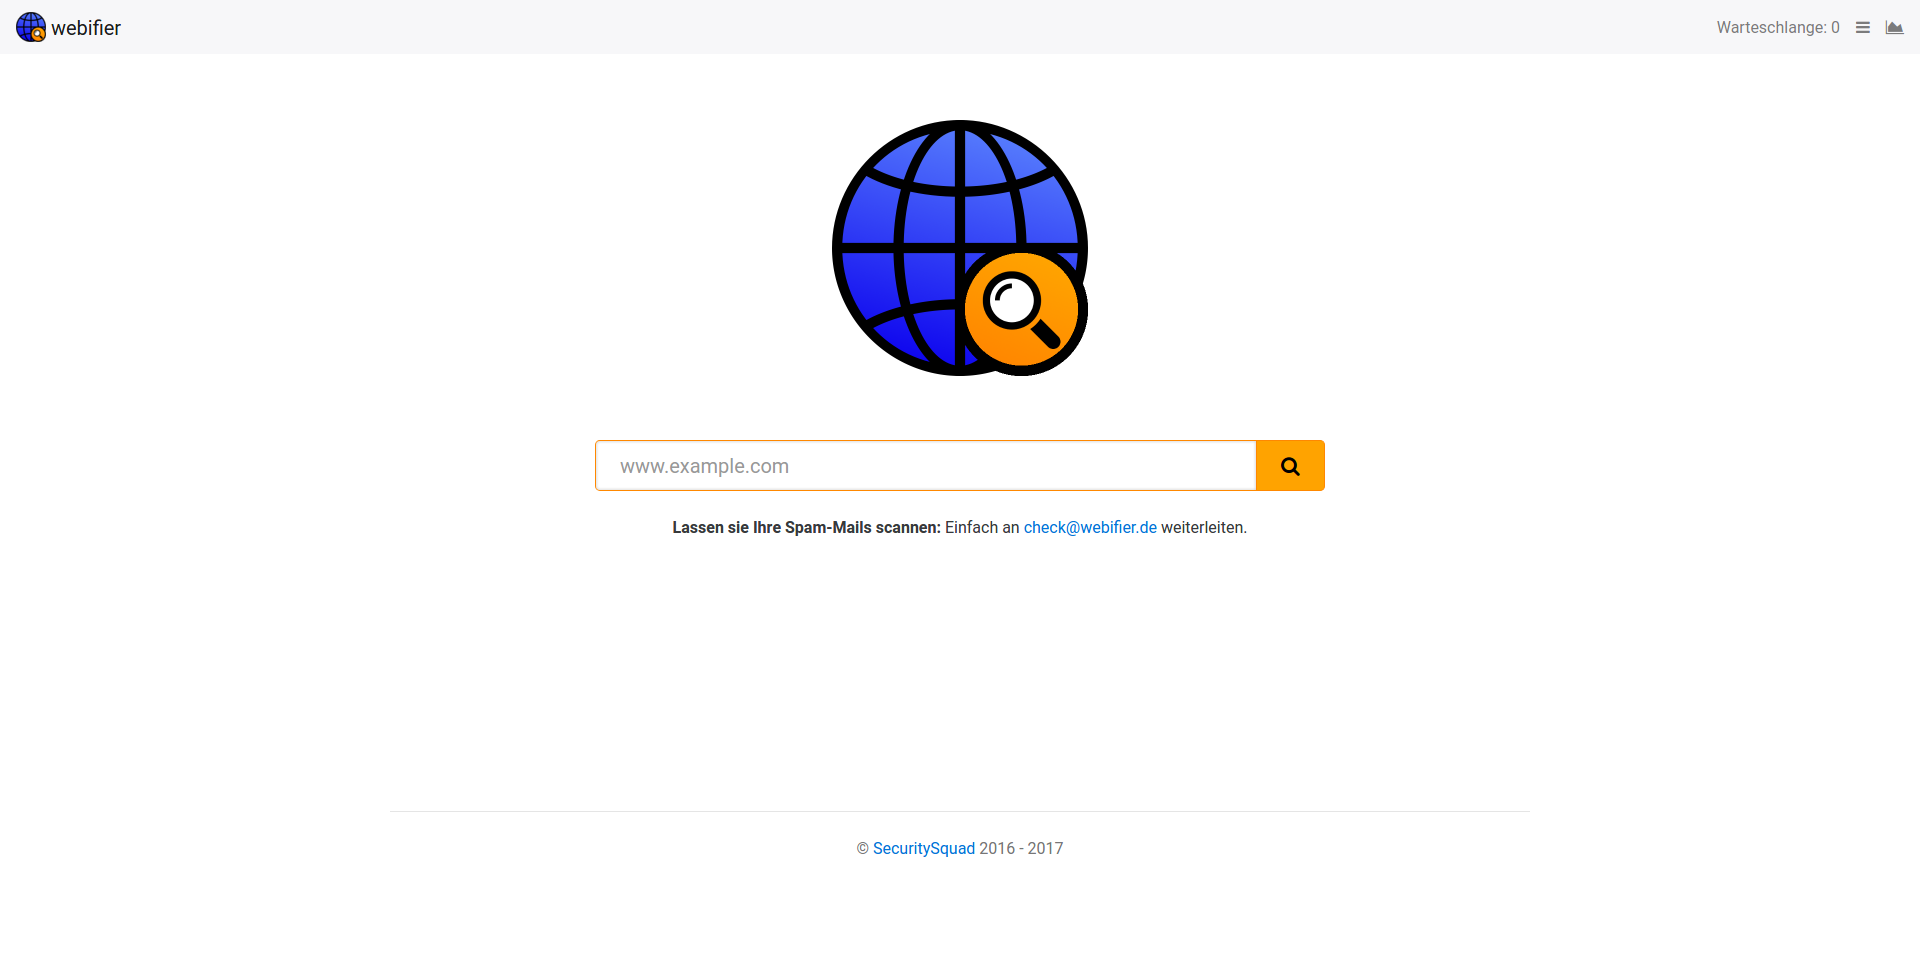
\includegraphics[width=\textheight]{images/platform/screenshot-start}
  \caption{webifier Platform - Startseite}
\end{figure}

\begin{figure}[H]
  \centering
  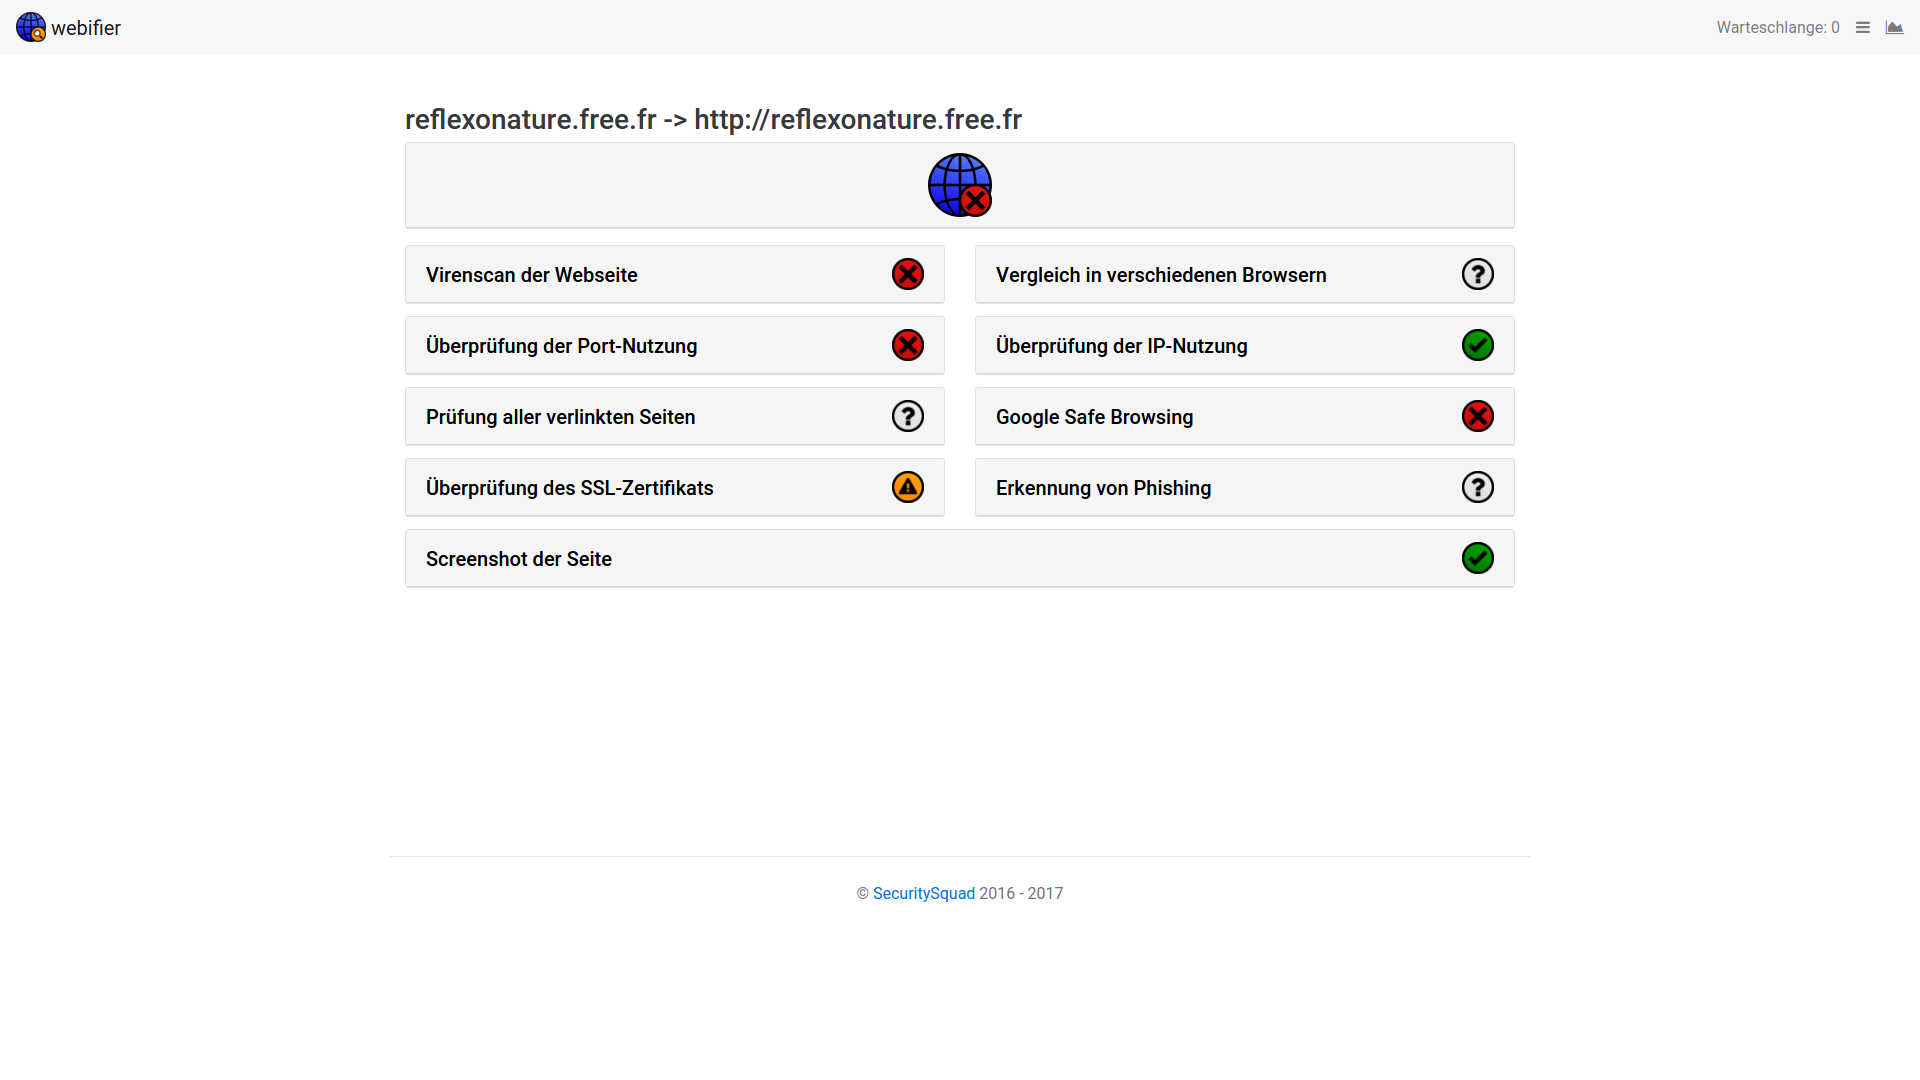
\includegraphics[width=\textheight]{images/platform/screenshot-reflexonature}
  \caption{webifier Platform - Ergebnisseite für reflexonature.free.fr}
  \label{fig:platform-result}
\end{figure}


\begin{figure}[H]
  \centering
  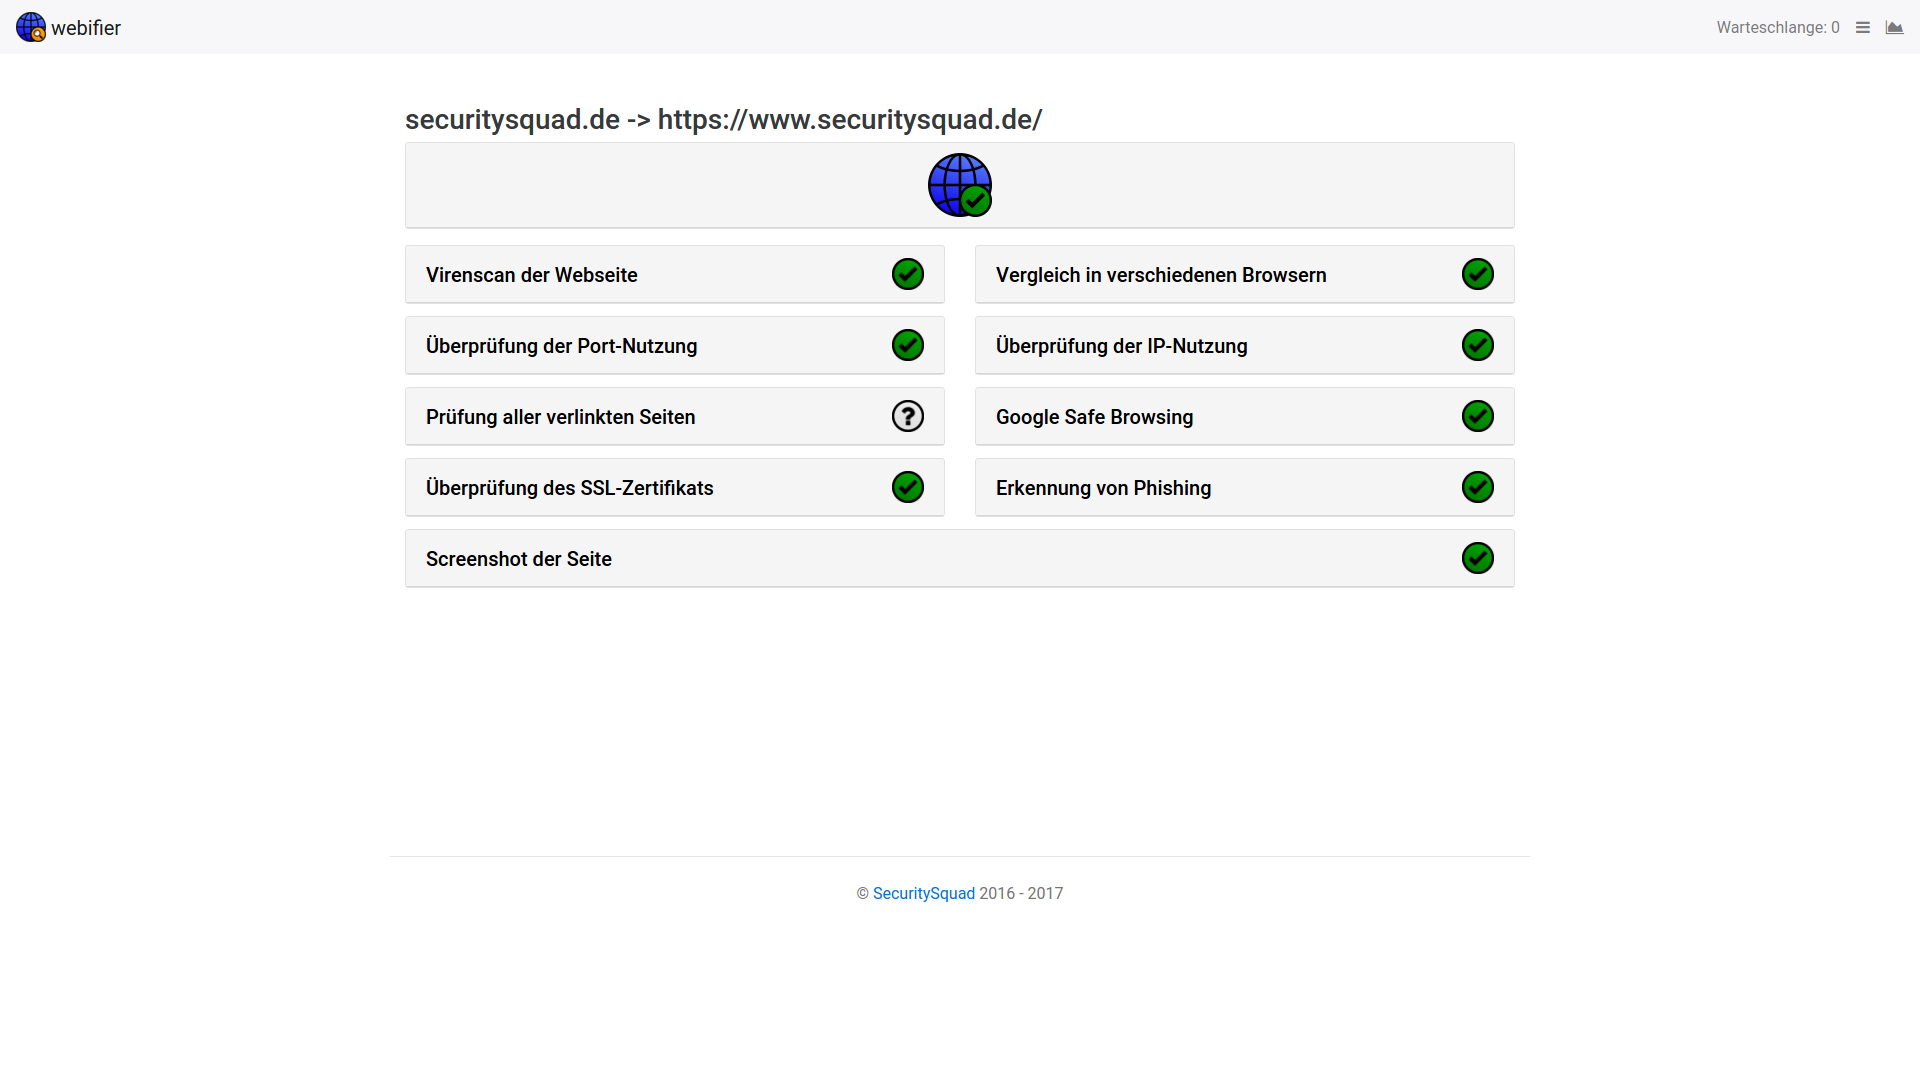
\includegraphics[width=\textheight]{images/platform/screenshot-securitysquad}
  \caption{webifier Platform - Ergebnisseite für securitysquad.de}
  \label{fig:platform-result}
\end{figure}


\begin{figure}[H]
  \centering
  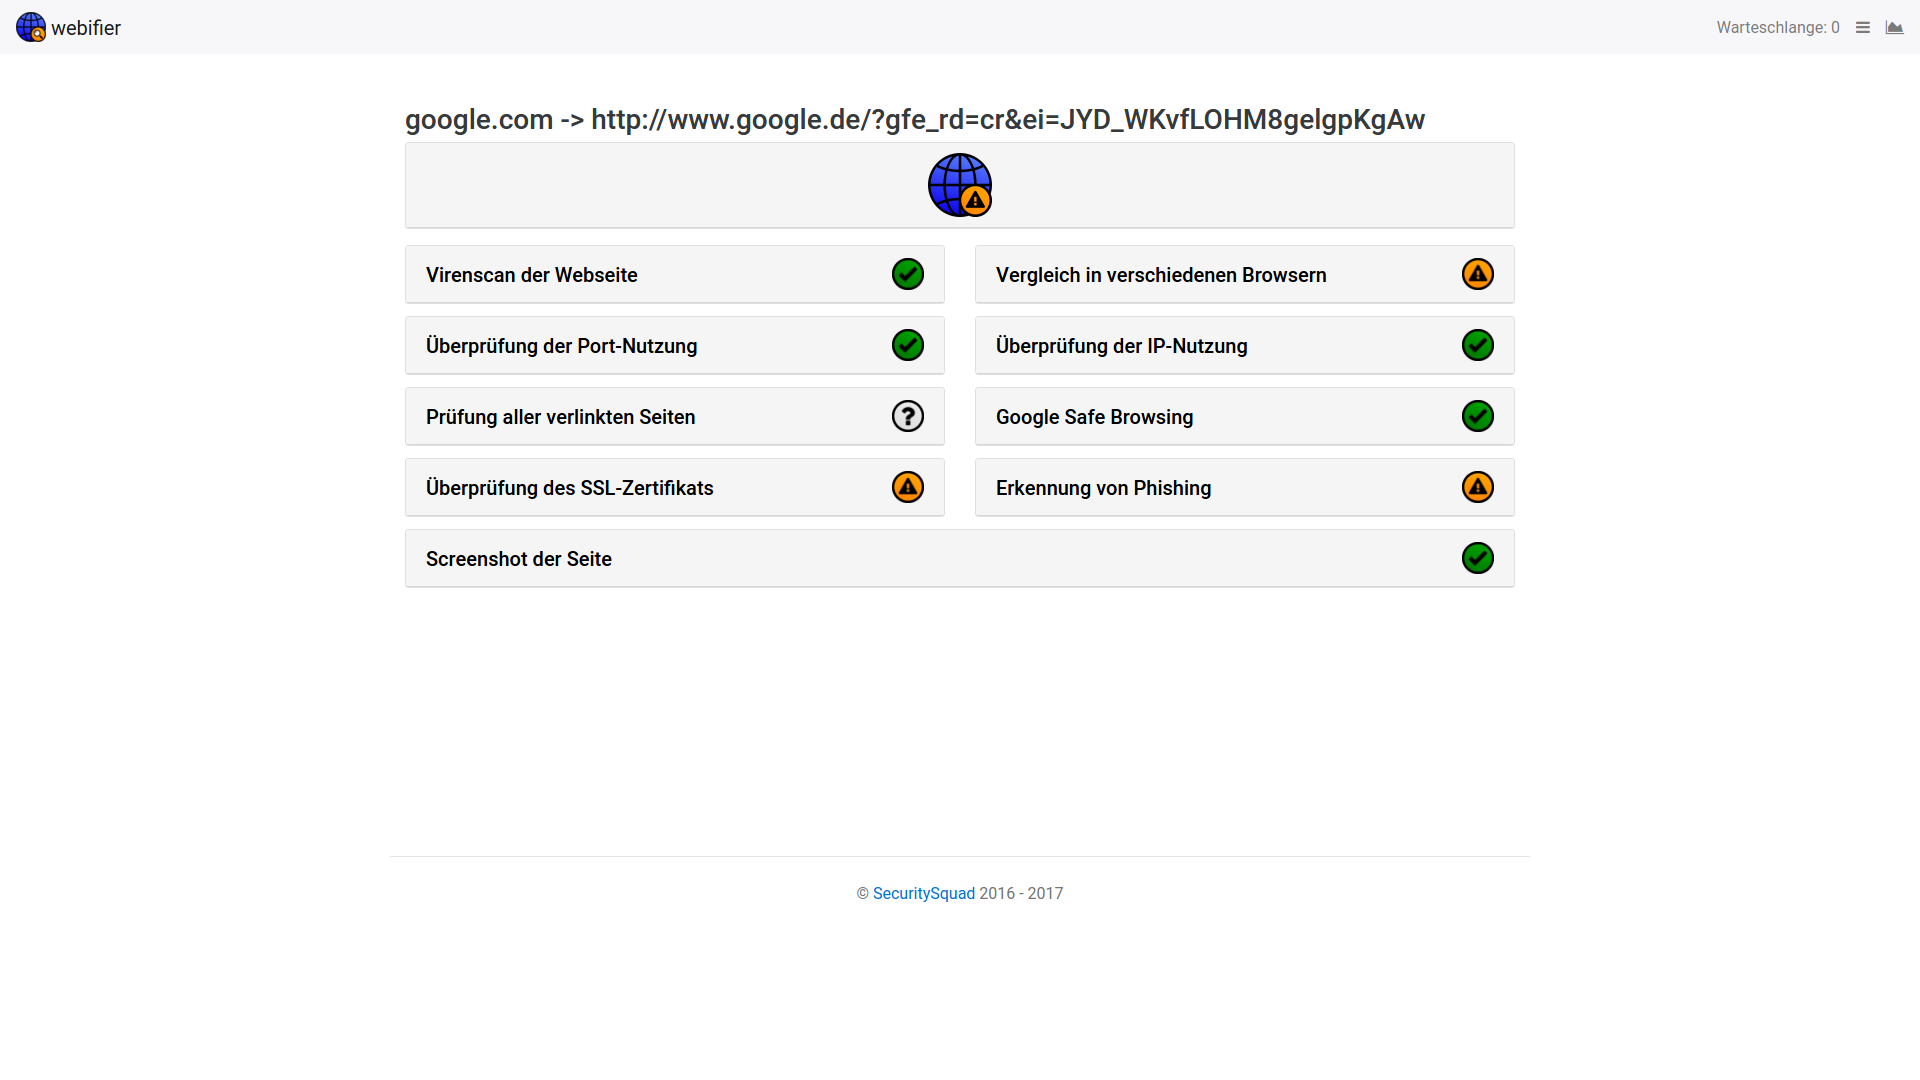
\includegraphics[width=\textheight]{images/platform/screenshot-google}
  \caption{webifier Platform - Ergebnisseite für google.com}
  \label{fig:platform-result}
\end{figure}


\end{landscape}

\newpage

\section*{TEIL E: Beispieldokumente webifierSingleTestResultData - webifier Data}
\label{app:e}

\begin{scriptsize}
\lstset{
    style=eclipsejavascript,
    caption={Beispieldokument webifierSingleTestResultData: Virenscan der Webseite - webifier Data},
}
\begin{lstlisting}
{
    "_id" : "2429f999-3168-4070-b085-7887ee64d8a0",
    "_class" : "de.securitysquad.webifier.persistence.domain.WebifierSingleTestResultData",
    "testId" : "61574eb4-e9ac-42e2-9140-4c1ce23a2891_5b8bcdbf-2d89-4930-915a-d65c5367bd28",
    "name" : "VirusScan",
    "startup" : "docker run --rm --name #ID -e URL=#URL -e ID=#ID webifier-test-virusscan",
    "shutdown" : "docker stop #ID",
    "enabled" : true,
    "weight" : 5,
    "startupTimeoutInSeconds" : 600,
    "shutdownTimeoutInSeconds" : 30,
    "result" : "MALICIOUS",
    "resultInfo" : {
        "scanned_files" : 4,
        "malicious_files" : 3,
        "suspicious_files" : 0,
        "files" : [
            {
                "name" : "index98e1.html",
                "result" : "MALICIOUS"
            },
            {
                "name" : "index-2.html",
                "result" : "CLEAN"
            },
            {
                "name" : "indexec9e.html",
                "result" : "MALICIOUS"
            },
            {
                "name" : "index3547.html",
                "result" : "MALICIOUS"
            }
        ]
    },
    "durationInMillis" : NumberLong(142805),
    "overallResult" : DBRef("webifierTestResultData", "82879e46-b286-4bdf-9876-875dc67e5708")
}
\end{lstlisting}
\end{scriptsize}

\newpage

\begin{scriptsize}
\lstset{
    style=eclipsejavascript,
    caption={Beispieldokument webifierSingleTestResultData: Vergleich in verschiedenen Browsern - webifier Data},
}
\begin{lstlisting}
{
    "_id" : "70210b9f-e4fc-475b-a40a-5c98f49a18d3",
    "_class" : "de.securitysquad.webifier.persistence.domain.WebifierSingleTestResultData",
    "testId" : "b19e3a9c-7bca-4d4f-b03b-a87e086d1592_2dd8aa86-b6b5-434a-a627-3ae11a0c1b9e",
    "name" : "HeaderInspection",
    "startup" : "docker run --rm --name #ID -e URL=#URL -e ID=#ID webifier-test-header-inspection",
    "shutdown" : "docker stop #ID",
    "enabled" : true,
    "weight" : 1,
    "startupTimeoutInSeconds" : 300,
    "shutdownTimeoutInSeconds" : 30,
    "result" : "MALICIOUS",
    "resultInfo" : {
        "medianRatio" : 0.9945236763609246,
        "worstRatio" : 0.993661446681581,
        "medianDiff" : 5522,
        "worstDiff" : 5589,
        "browsers" : [
            "Android 4.3",
            "Android 5.1",
            "iPhone 6, iOS 8.4",
            "iPhone 6, iOS 9.3",
            "Windows 10, Chrome 54.0",
            "Windows XP, Internet Explorer 6.0",
            "Windows XP, Firefox 4.0",
            "OS X 10.11, Safari 10.0",
            "OS X 10.11, Safari 6.0"
        ]
    },
    "durationInMillis" : NumberLong(137104),
    "overallResult" : DBRef("webifierTestResultData", "77f77195-f32e-4305-bff3-c29893a4d2f5")
}
\end{lstlisting}
\end{scriptsize}

\newpage

\begin{scriptsize}
\lstset{
    style=eclipsejavascript,
    caption={Beispieldokument webifierSingleTestResultData: Überprüfung der Port-Nutzung - webifier Data},
}
\begin{lstlisting}
{
    "_id" : "8908d41a-449d-4760-a9a2-32e6603dc6f1",
    "_class" : "de.securitysquad.webifier.persistence.domain.WebifierSingleTestResultData",
    "testId" : "ff4109af-6e5a-4824-ae6a-93d4a06b9077_6b9f0762-92ea-452a-a10f-e469f7884591",
    "name" : "PortScan",
    "startup" : "docker run --rm --name #ID -e URL=#URL -e ID=#ID webifier-test-portscan",
    "shutdown" : "docker stop #ID",
    "enabled" : true,
    "weight" : 3,
    "startupTimeoutInSeconds" : 300,
    "shutdownTimeoutInSeconds" : 30,
    "result" : "SUSPICIOUS",
    "resultInfo" : {
        "unknown_ports" : [
            22
        ]
    },
    "durationInMillis" : NumberLong(12740),
    "overallResult" : DBRef("webifierTestResultData", "d15e97c7-3687-4261-b1f1-549ba94666ef")
}
\end{lstlisting}
\end{scriptsize}

\begin{scriptsize}
\lstset{
    style=eclipsejavascript,
    caption={Beispieldokument webifierSingleTestResultData: Überprüfung der IP-Nutzung - webifier Data},
}
\begin{lstlisting}
{
    "_id" : "2c0b3f33-b120-4b74-b9a1-75ac9d1ad269",
    "_class" : "de.securitysquad.webifier.persistence.domain.WebifierSingleTestResultData",
    "testId" : "33e76954-dc94-48a9-a816-99ddeb647887_8cae7586-8360-4d6b-a855-343a23aff0df",
    "name" : "IpScan",
    "startup" : "docker run --rm --name #ID -e URL=#URL -e ID=#ID webifier-test-ipscan",
    "shutdown" : "docker stop #ID",
    "enabled" : true,
    "weight" : 3,
    "startupTimeoutInSeconds" : 300,
    "shutdownTimeoutInSeconds" : 30,
    "result" : "CLEAN",
    "resultInfo" : {
        "risky_hosts" : [ ]
    },
    "durationInMillis" : NumberLong(9803),
    "overallResult" : DBRef("webifierTestResultData", "e3d35b18-332d-4c16-b1a9-d116850509e9")
}

\end{lstlisting}
\end{scriptsize}

\newpage

\begin{scriptsize}
\lstset{
    style=eclipsejavascript,
    caption={Beispieldokument webifierSingleTestResultData: Prüfung aller verlinkten Seiten - webifier Data},
}
\begin{lstlisting}
{
    "_id" : "4d3362e0-e22a-4daa-a7e9-bee4151d1e04",
    "_class" : "de.securitysquad.webifier.persistence.domain.WebifierSingleTestResultData",
    "testId" : "cf7fb17e-edfa-4f44-91cf-ebc60a5e67f6_d63a0f52-ba63-45fb-b9f1-9e51f3639de3",
    "name" : "LinkChecker",
    "startup" : "docker run --rm --name #ID -e URL=#URL -e ID=#ID webifier-test-linkchecker",
    "shutdown" : "docker stop #ID",
    "enabled" : true,
    "weight" : 1,
    "startupTimeoutInSeconds" : 300,
    "shutdownTimeoutInSeconds" : 30,
    "result" : "MALICIOUS",
    "resultInfo" : {
        "hosts" : [
            {
                "host" : "alt.com",
                "result" : "MALICIOUS"
            },
            {
                "host" : "adultfriendfinder.com",
                "result" : "UNDEFINED"
            },
            {
                "host" : "outpersonals.com",
                "result" : "UNDEFINED"
            },
            {
                "host" : "cams.com",
                "result" : "CLEAN"
            },
            {
                "host" : "accounts.google.com",
                "result" : "SUSPICIOUS"
            },
            {
                "host" : "secureimage.securedataimages.com",
                "result" : "UNDEFINED"
            },
            {
                "host" : "fonts.gstatic.com",
                "result" : "UNDEFINED"
            }
        ]
    },
    "durationInMillis" : NumberLong(4512),
    "overallResult" : DBRef("webifierTestResultData", "822bde3c-92bc-4980-8ef9-7f07fce49d57")
}
\end{lstlisting}
\end{scriptsize}

\newpage

\begin{scriptsize}
\lstset{
    style=eclipsejavascript,
    caption={Beispieldokument webifierSingleTestResultData: Google Safe Browsing - webifier Data},
}
\begin{lstlisting}
{
    "_id" : "0ba4f3e3-ff1a-4056-b2e4-87028af128c1",
    "_class" : "de.securitysquad.webifier.persistence.domain.WebifierSingleTestResultData",
    "testId" : "7872a958-9e3b-4c44-bd02-38665e06edd5_61c8deb7-80ed-400c-b4d7-64645201397d",
    "name" : "GoogleSafeBrowsing",
    "startup" : "docker run --rm --name #ID -e URL=#URL -e ID=#ID -e API_KEY=XYZ webifier-test-google-safe-browsing",
    "shutdown" : "docker stop #ID",
    "enabled" : true,
    "weight" : 3,
    "startupTimeoutInSeconds" : 300,
    "shutdownTimeoutInSeconds" : 30,
    "result" : "MALICIOUS",
    "resultInfo" : {
        "matches" : [
            "http://www.pizzotti.net/",
            "http://heirem-art.de/crpzw3bh.php?id=19579352",
            "http://mardhavi.com/krmvcpgg.php?id=19346074",
            "http://mardhavi.com/krmvcpgg.php?id=19346073"
        ]
    },
    "durationInMillis" : NumberLong(5709),
    "overallResult" : DBRef("webifierTestResultData", "9f362427-d34a-456a-b72b-919f26e5de40")
}
\end{lstlisting}
\end{scriptsize}

\newpage

\begin{scriptsize}
\lstset{
    style=eclipsejavascript,
    caption={Beispieldokument webifierSingleTestResultData: Überprüfung des SSL-Zertifikats - webifier Data},
}
\begin{lstlisting}
{
    "_id" : "d1aec3e7-139e-41f8-ab4b-9f4cfd3d382e",
    "_class" : "de.securitysquad.webifier.persistence.domain.WebifierSingleTestResultData",
    "testId" : "d712d875-da26-4ecf-a81a-66f902644067_173cc3bd-71c3-445e-939f-e234deb24b2a",
    "name" : "CertificateChecker",
    "startup" : "docker run --rm --name #ID -e URL=#URL -e ID=#ID webifier-test-certificatechecker",
    "shutdown" : "docker stop #ID",
    "enabled" : true,
    "weight" : 3,
    "startupTimeoutInSeconds" : 300,
    "shutdownTimeoutInSeconds" : 30,
    "result" : "CLEAN",
    "resultInfo" : {
        "certificate" : {
            "subject" : {
                "name" : "www.paypal.com",
                "organisation" : "PayPal, Inc.",
                "organisation_unit" : "CDN Support"
            },
            "issuer" : {
                "name" : "Symantec Class 3 EV SSL CA - G3",
                "organisation" : "Symantec Corporation",
                "organisation_unit" : "Symantec Trust Network"
            },
            "validity" : {
                "from" : NumberLong("1454371200000"),
                "to" : NumberLong("1509407999000")
            },
            "return_code" : "0 (ok)"
        }
    },
    "durationInMillis" : NumberLong(995),
    "overallResult" : DBRef("webifierTestResultData", "e8d3cc31-1140-4efd-a11b-cd501ad19952")
}
\end{lstlisting}
\end{scriptsize}

\newpage

\begin{scriptsize}
\lstset{
    style=eclipsejavascript,
    caption={Beispieldokument webifierSingleTestResultData: Erkennung von Phishing - webifier Data},
}
\begin{lstlisting}
{
    "_id" : "6ebf08e4-7d3b-49ce-be02-76599ffca44d",
    "_class" : "de.securitysquad.webifier.persistence.domain.WebifierSingleTestResultData",
    "testId" : "138a8a96-3b80-42aa-93eb-365a82ee2b85_718c9b2d-3e82-4638-a596-cd9b3486b2c7",
    "name" : "PhishingDetector",
    "startup" : "docker run --rm --name #ID -e URL=#URL -e ID=#ID webifier-test-phishingdetector",
    "shutdown" : "docker stop #ID",
    "enabled" : true,
    "weight" : 5,
    "startupTimeoutInSeconds" : 300,
    "shutdownTimeoutInSeconds" : 30,
    "result" : "MALICIOUS",
    "resultInfo" : {
        "keywords" : [
            "paypal",
            "bezahlen",
            "senden",
            "oder"
        ],
        "matches" : [
            {
                "url" : "https://www.paypal.com/de/home",
                "result" : "MALICIOUS",
                "ratio" : 0.9989644191977116,
                "html_ratio" : 0.9958576767908464,
                "content_ratio" : 1,
                "screenshot_ratio" : 1,
                "comparison" : null
            },
            {
                "url" : "https://www.paypal.com/de/webapps/mpp/home",
                "result" : "MALICIOUS",
                "ratio" : 0.9990458916024976,
                "html_ratio" : 0.9961835664099902,
                "content_ratio" : 1,
                "screenshot_ratio" : 1,
                "comparison" : null
            }
        ]
    },
    "durationInMillis" : NumberLong(157961),
    "overallResult" : DBRef("webifierTestResultData", "cf39cafb-8e2e-4a86-9497-e4fe60e5f996")
}

\end{lstlisting}
\end{scriptsize}


\end{document}
